\documentclass{book}  % fundamental class file is 'book'.
\usepackage{piers}  % use the file 'piers.sty'.
\pagestyle{piers}


\usepackage{hyperref}
\usepackage{cite}
\usepackage{amsmath}
%\interdisplaylinepenalty=2500 % suggested by IEEE to use with amsmath package
\usepackage{amsfonts}
\usepackage{graphicx}
\usepackage{caption}
\usepackage{subcaption}
\usepackage{epstopdf}

\usepackage[T1]{fontenc} % optional
\usepackage[cmintegrals]{newtxmath}
\usepackage{bm} % optional


% ================ self-defined command ==================
\usepackage{color} % for marking text
\newcommand{\highlight}[1]{\Huge\textcolor{red}{XG : #1}\normalsize}
\newcommand{\cphighlight}[1]{\Huge\textcolor{blue}{CP : #1}\normalsize}
\newcommand{\defaultfigurewidth}{0.5\columnwidth}
% --------- fix non-conventional piers command -----------
% So you can simply use abstract, section, and subsection
% as used in IEEE papers.
\newenvironment{abstract}{\begin{piersabstract}}{%
	\end{piersabstract}\ignorespacesafterend% as suggested above
}
\renewcommand{\section}[1]{\psection{#1}}
\renewcommand{\subsection}[1]{\psubsection{#1}}


% correct bad hyphenation here
\hyphenation{op-tical net-works semi-conduc-tor}

\begin{document}

\title{Design of High Speed Link System}
\maketitle

%=== List of authors (in order) ========
%-- Author(s) for the first affiliation ---
\author      {Chang-Pao Chang}
\affiliation {University of Illinois at Urbana-Champaign}
\address     {}% optional
\city        {Urbana}
\postalcode  {61801} % optional
\country     {USA}
\phone       {} % optional
\fax         {} % optional
\email       {cchang95@uiuc.com}  % optional
\misc        { }  % optional
\nomakeauthor
%------------------------------------

%=== List of authors (in order) ========
%-- Author(s) for the second affiliation ---
\author      {Xiou Ge}
\affiliation {University of Illinois at Urbana-Champaign}
\address     {}% optional
\city        {Urbana}
\postalcode  {61801} % optional
\country     {USA}
\phone       {} % optional
\fax         {} % optional
\email       {xiouge2@uiuc.com}  % optional
\misc        { }  % optional
\nomakeauthor
%-------------------------------------

%---Output of Authors----------------------
\begin{authors}	
	{\bf Chang-Pao Chang}$^{1}$, {\bf Xiou Ge}$^{2}$\\
	\medskip
	$^{1}$cchang95@illinois.edu\\
	$^{2}$xiouge2@illinois.edu	
\end{authors}
%--------------------------


%---Content of Paper Abstract-----------------------
\begin{paper}
	
\begin{abstract}
A high speed data link with total length over twenty inches is proposed in this paper. With feed forward equalizer (FFE), and decision feed-back equalizer(DFE), the data rate can goes up to 20Gbps. The passive channel consists of bonding wire for package to printed circuit board (PCb) transition, total 12 inches of PCB lines, and two top-to-bottom via transition in PCB. With carefully designed matching network for each discontinuity, the overall performance of passive channel has -5dB insertion loss at 10GHz. Combined with DFE and FFE, the resulting eye has 98\% eye width and 92\% eye height at 3Gbps, and 66\% eye width and 81.5\% eye height at 20Gbps. 

\cphighlight{Do you need PDA?}
\end{abstract}

\section{Introduction}
With increasing speed, the urgent demand on higher performance for high speed link has become a critical problem in signal integrity. High-speed backplane serial I/O interconnections such as PCI-Express \cite{na_welcome_pcisig}, Serial ATA (SATA) \cite{I_serial_ata}, Thunderbolt \cite{na_thunderbolt_technology} amazed us years ago. However, the dawning mobile age shows even higher demand on high speed data link. Fig.~\ref{fig:pcie_speed} shows the increasing data rate of PCI Express \cite{na_welcome_pcisig}. \\

\begin{figure}[htbp!]
	\centering
	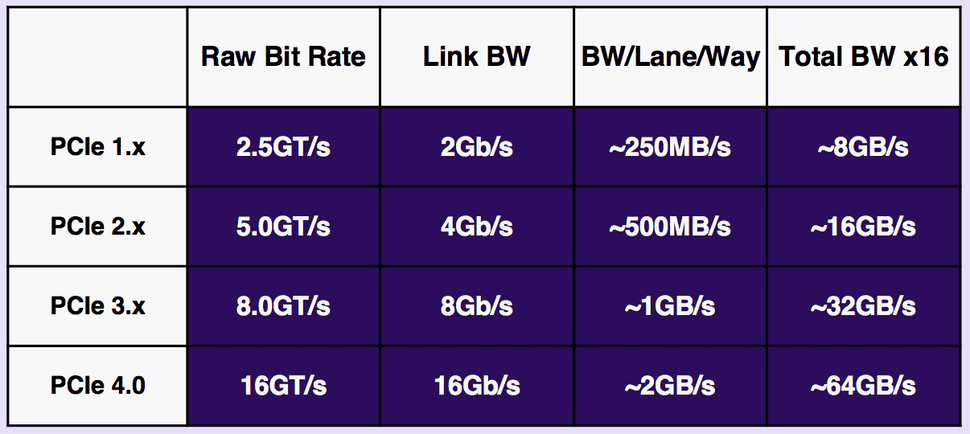
\includegraphics[width=0.8\columnwidth]{./img/pcie-4-0-bandwidth.png}
	\caption{Data rate of PCI Express in different generations \cite{C_doublespeed_nextgen}.}
	\label{fig:pcie_speed}
\end{figure}

To improve the signal integrity (SI) of high speed link, several techniques has been proposed. Matching network, passive equalizers, analog equalizers, and digital equalizers were proposed in several different scenarios. However, because fo simplicity, FFE and DFE are the two most used finite impulse response (FIR) filter to equalize the desired channel.

This report is organized as follow, first we will give a system level preview. Then the design procedure of channel and equalizers are described in following sections. Finally the overall systems will be simulated in Cadence Virtuoso. 


\section{System Level Design}
\label{sec:system}
The high speed link we built consists of three main subsystems, namely the transmitter (TX) block, the channel block and the receiver (RX) block. Two paths are designed to transmit the bit stream and the clock signal separately. 

In the TX block, signal path is composed of a data transmitter and a feed-forward equalizer (FFE) implemented with Verilog, whereas the clock path has a clock transmitter connected to the external clock generator. Both transmitters can be implemented using transistor level inverters.

The channel block consists of bonding wire and the actual signal traces. Since the channel we built is largely symmetric, in order to speed up the simulation, we adopt 'divide and conquer' strategy. We split our channel into 24 small blocks. It turns out that there are only four distinct type of structures we need to simulate, namely the PCB trace, the via transition, package trace and bonding wire transition. After obtaining the S-parameter data for each individual block, we cascade the S-parameter using Keysight ADS and quickly obtain the S-parameter for the entire channel. 

\begin{figure}[htbp!]
	\centering
	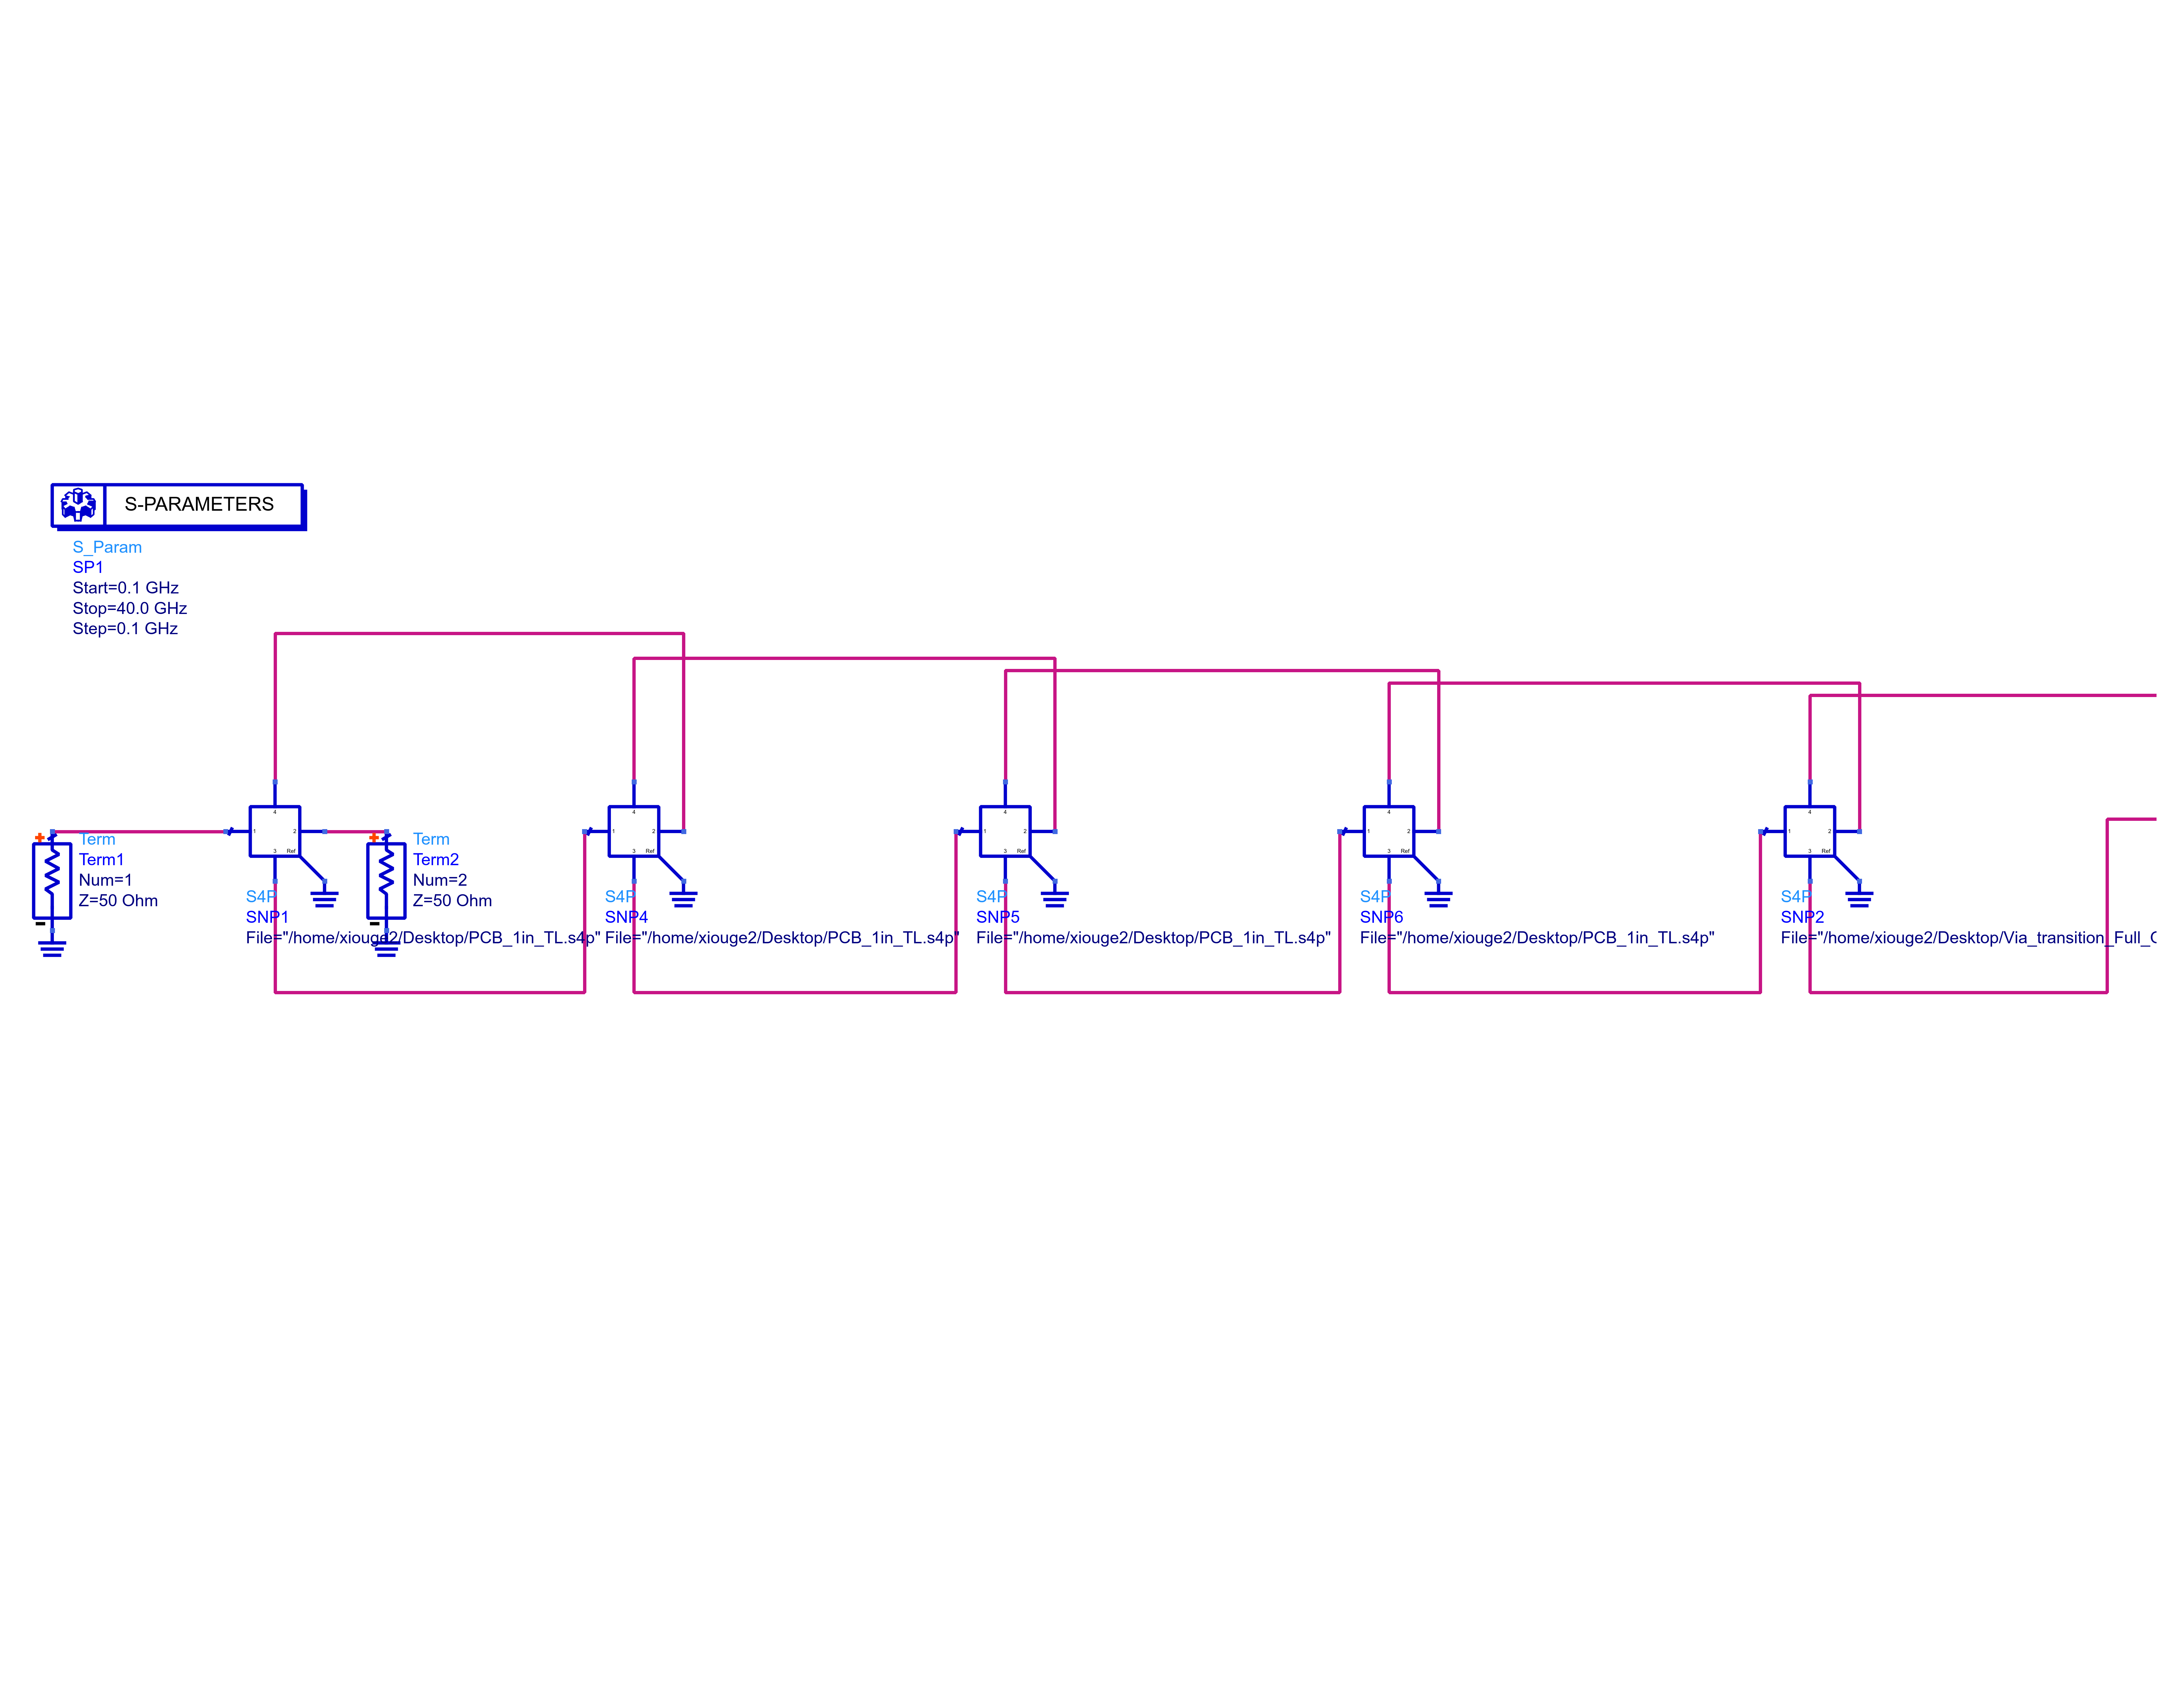
\includegraphics[width=0.8\columnwidth]{./img/cascade_schematics.png}
	\caption{Partial ADS Schematics for S-parameter Cascade.}
\end{figure}

In the RX block, signal path is composed of a transistor level data amplifier to make up for signal loss in the channel, and a decision feedback equalizer (DFE) implemented with Verilog. Whereas the clock path has a transistor level clock amplifier and a Verilog clock deskew block. Decision output from the DFE will be the output for the RX block and the entire high speed link.

To test the system, a random bit stream is generated using the PRBS unit in Cadence Virtuoso and fed into the input of FFE in the TX block. Eye diagrams at the input of channel, input and output of the DFE are plotted to evaluate performance of the high speed link.


\section{Channel Design}
\label{sec:channel_design}

Since the target bit rate is quite high (3Gbps), we used one of the low loss substrate to design our PCB. The RO4003 from Rogers company is widely used to design various high frequency circuit \cite{na_ro4003_rogers}. We use PCB of 9 layers of metal. Fig.~\ref{fig:pcb_layers} shows the dimensions of each layers. The top and bottom layer are the signal layer, and the rest 7 layers at the middle of the PCB are simulated as ground layer. These ground layers were later connected using grounded vias. Each layer is of 19 mil height, and the thickness of metal is 1 mil. \\

As for package, we use one layer of thin-film ceramic from Murawa \cite{na_alumina_substratess}. The substrate is far more thinner than those used in PCB. Table.~\ref{table:material} shows the material properties used for PCB and package.

\begin{table}[h]
	\renewcommand{\arraystretch}{1.3}
	\begin{center}
		\begin{tabular}{| l | l | l | c | c | c |}
			\hline
			Usage   & Substrate  & Trace & Metal Layers & $\varepsilon_r$ & $\tan\delta$ \\ \hline
			PCB     & RO4003  \cite{na_ro4003_rogers} & Copper & 9 & 3.8 & 0.02  \\ \hline
			Package & Alumina \cite{na_alumina_substratess} & Copper & 2 & 9.8 & 0.02 \\
			\hline
		\end{tabular}
	\end{center}
	\label{table:material}
	\caption{Material properties used for channel design.}
	\vskip0.2in
\end{table}

\subsection{PCB Traces}
\label{subsec:pcb_traces}
The differential PCB traces are designed such that the single line impedance is 50 $\Omega$, and the differential impedance is 100 $\Omega$. Fig.~\ref{fig:pcb_trace} and Table.~\ref{table:pcb_trace} shows the design parameters to achieve the desired impedance. The 2D extraction tool, Ansys Q2D is used to analyze and fine-tune the parameters. Fig.~\ref{fig:pcb_trace_impedance} shows the impedance of the differential line up to 40GHz. It shows that the differential impedance is 96$\Omega$ while the common impedance is 25$\Omega$ at 10GHz. 

\begin{table}[htbp!]
	\renewcommand{\arraystretch}{1.3}	
	\begin{center}
		\begin{tabular}{| c | c | c | c | c | c | c | c |}
			\hline
			Parameters  & Value  & Parameters & Value  & Parameters & Value  & Parameters & Value \\ \hline
			$W_{PCB}$   & 40 mil & $D_{PCB}$  & 80 mil & $H_{PCB}$  & 19 mil & $T_{PCB}$  & 1 mil \\
			\hline
		\end{tabular}
	\end{center}
	\label{table:pcb_trace}
	\caption{Design parameter of PCB trace.}
	\vskip0.2in
\end{table}

\begin{figure}[htbp!]
	\centering
	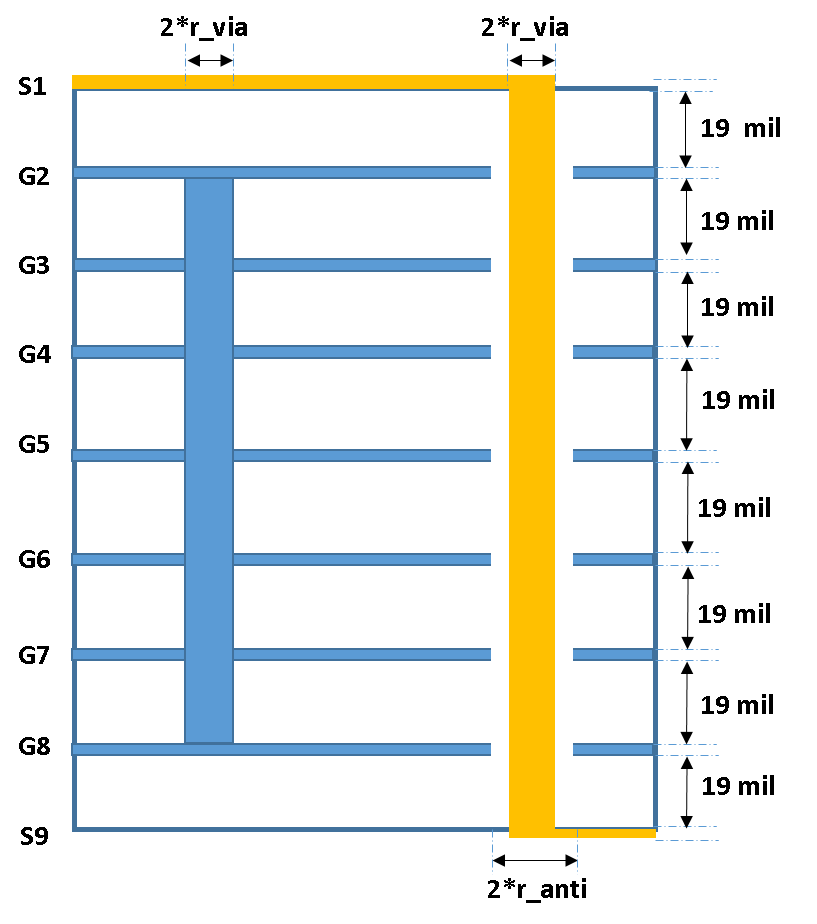
\includegraphics[width=0.8\columnwidth]{./img/PCB/PCB_layer_dimension.png}
	\caption{Dimension and layers in designated PCB. $r\_via=20 mil$ is the radius of both signal and ground via. The height of each PCB layer is 19 mil, and the thickness of copper is 1 mil. }
	\label{fig:pcb_layers} % label must put at the last
\end{figure}

\begin{figure}[htbp!]
	\centering
	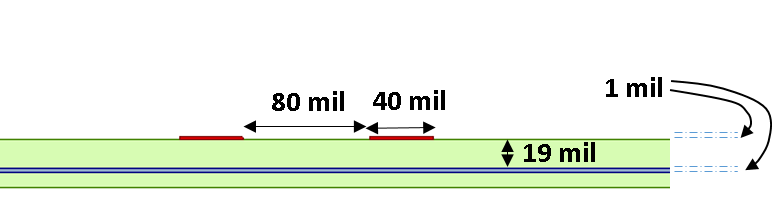
\includegraphics[width=0.8\columnwidth]{./img/PCB/differential_PCB_2D_CrossSection.png}
	\caption{Design parameter of PCB traces.}
	\label{fig:pcb_trace} % label must put at the last
\end{figure}

\begin{figure}[htbp!]
	\centering
	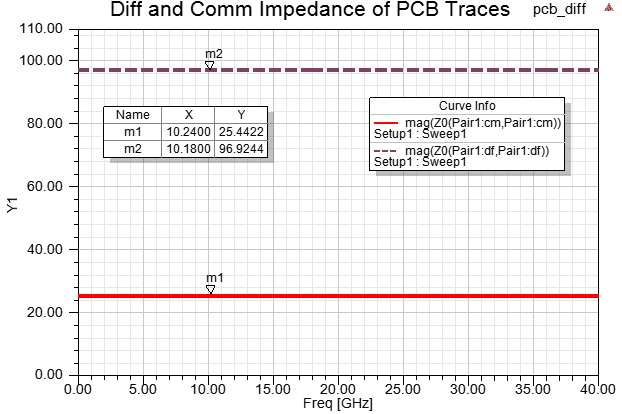
\includegraphics[width=0.8\columnwidth]{./img/PCB/differential_PCB_2D_impedance.png}
	\caption{Differential and common impedance of designated PCB traces. Solid: common mode impedance; dash: differential mode impedance.}
	\label{fig:pcb_trace_impedance} % label must put at the last
\end{figure}


\subsection{Via Transition}
\label{subsec:via_tran}
Since there will be a via transition from top to the bottom of the PCB, the strong discontinuity of this via transition will cause strong reflection, as shown in Fig.~\ref{fig:pcb_layers}. The entire structure, however, can be modeled using quasi-static approach. The via itself can be modeled as lumped resistance and inductance, and the parasitic capacitance distributed around the via to the ground plane surrounded. Fig.~\ref{fig:pcb_via_lump} shows the quasi-static models of via transition, and Fig.~\ref{fig:pcb_via_lump_model} shows the lumped model of via transition of differential line. \\

The 3D quasi-static extraction tool Ansys Q3D \cite{na_ansys_q3d} is used to extract the lumped element of these conductor. Fig.~\ref{fig:pcb_via_tran_Q3D} shows the via transition model for Q3D extraction. Since the structure is symmetry, to lower the reflection, a simple approximation can be used. The lumped differential impedance defined in \ref{eq:pcb_via_tran_lump_diff} is set to be 100 $\Omega$. This can be achieved through adjusting the radius of anti-pad, $r\_anti$ in Fig.~\ref{fig:pcb_layers}.

\begin{equation}\label{eq:pcb_via_tran_lump_diff}
Z^{lump}_{diff}\equiv \sqrt{\frac{L_{11} - L_{12}}{C_{11} + \left|C_{12}\right|}} = 100\Omega
\end{equation}

\begin{figure*}[htbp!]
	\centering	
	\begin{minipage}[b]{0.5\linewidth}
		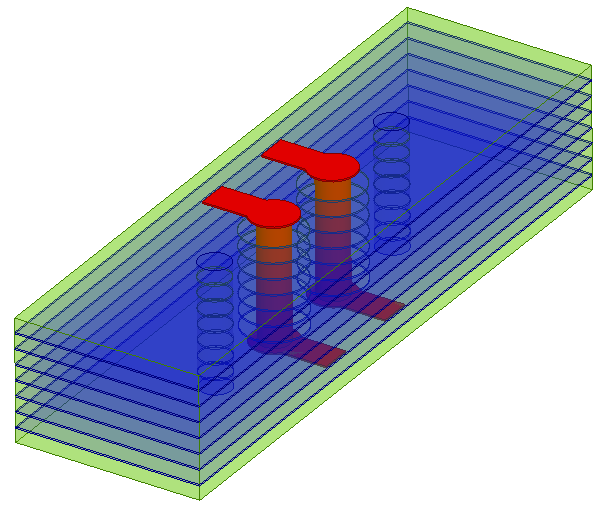
\includegraphics[width=\textwidth]{./img/PCB/Via_Transition/Q3D_tuned_side.png}
		\subcaption{Via transition simulated in Q3D for lumped element extraction.}
		\label{fig:pcb_via_tran_Q3D}
	\end{minipage}%
	\begin{minipage}[b]{0.5\linewidth}
		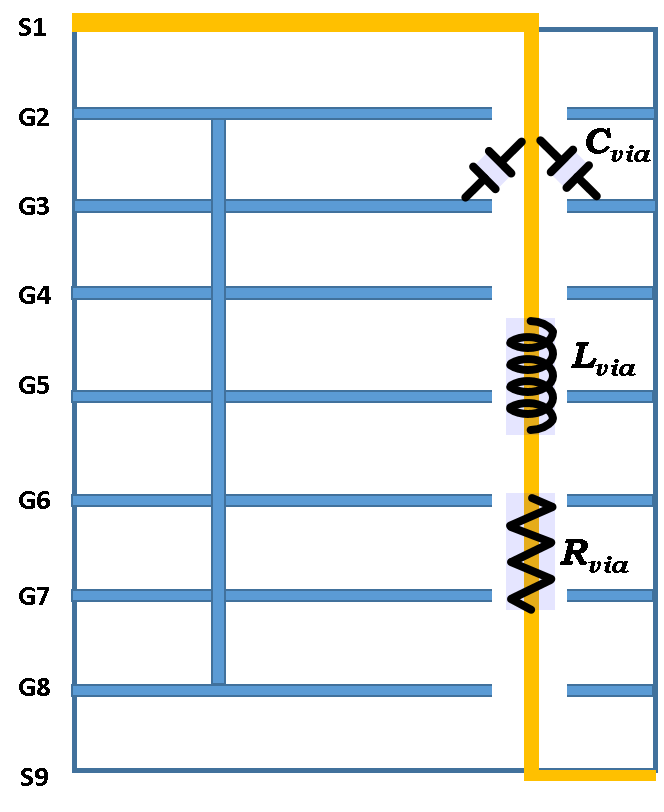
\includegraphics[width=\textwidth]{./img/PCB/Via_Transition/Via_transition_LC_modeling.png}
		\subcaption{Lumped model of via transition.}
		\label{fig:pcb_via_lump}
	\end{minipage}
	\begin{minipage}[b]{\linewidth}
		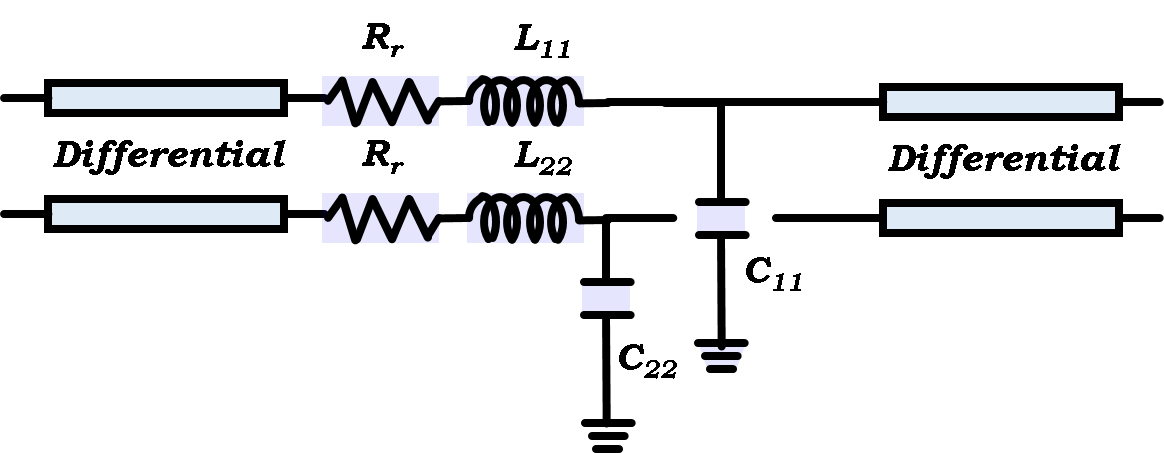
\includegraphics[width=\textwidth]{./img/PCB/Via_Transition/lumped_model.png}
		\subcaption{Lumped model of via transition.}
		\label{fig:pcb_via_lump_model}
	\end{minipage}
	\caption{Via transition model for Q3D extraction.}	
	\vskip0.2in	
\end{figure*}

\begin{table}[htbp!]
	\renewcommand{\arraystretch}{1.3}	
	\begin{center}
		\begin{tabular}{| c | c | c | c | c | c | c | c |}
			\hline
			Parameters  & Value  & Parameters & Value  \\ \hline
			$R_{Anti}$  & 75 mil & $R_{Via}$  & 20 mil \\
			\hline
		\end{tabular}
	\end{center}
	\label{table:pcb_via_tran}
	\caption{Design parameter of PCB trace.}
\end{table}
%
The preliminary result given in Q3D is later imported into HFSS for full-wave simulation. To eliminate the higher order mode around the discontinuity,  1 inch of microstrips are attached at both end of vias. Fig.~\ref{fig:pcb_via_trans_HFSS} shows the structure used in HFSS, and Fig.~\ref{fig:pcb_via_tran_S} shows the S parameter of differential and common mode. The high level of $S^{cc}_{11}$ shows good common mode rejection, around -10dB, below 10GHz, while the $S^{dd}_{11}$ remains below -20dB below 10 GHz. Fig.~\ref{fig:pcb_via_tran_Sdd11_smith} shows the smith chart of $S^{dd}_{11}$. The low reflection of differential mode can be observed that the reflection is below 0.26 with 10 GHz.

\begin{figure*}[htbp!]
	\centering	
	\begin{minipage}[b]{0.5\linewidth}
		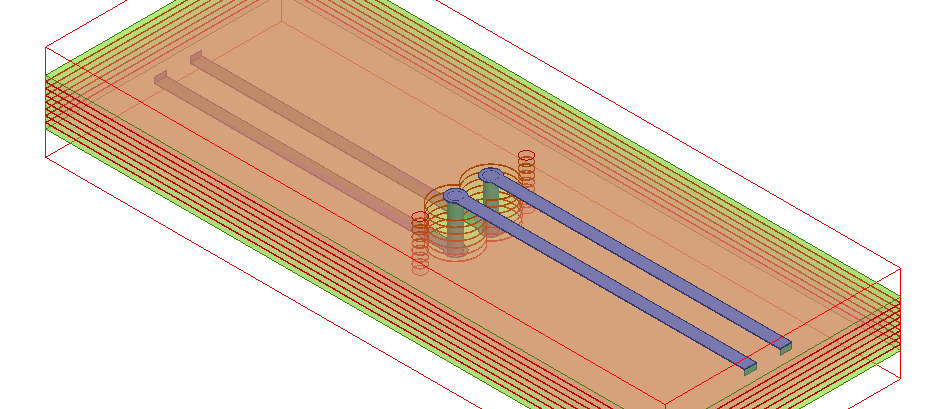
\includegraphics[width=\textwidth]{./img/PCB/Via_Transition/View_45_Degree.png}
		\subcaption{Tilted view.}
	\end{minipage}%
	\begin{minipage}[b]{0.5\linewidth}
		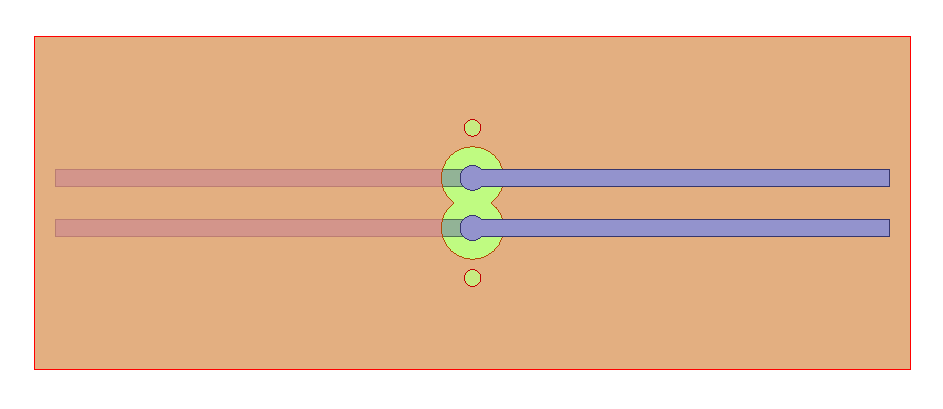
\includegraphics[width=\textwidth]{./img/PCB/Via_Transition/View_Top.png}
		\subcaption{Top view.}
	\end{minipage}
	\caption{Via transition simulated in HFSS.}
\end{figure*}

\begin{figure}[htbp!]
	\centering
	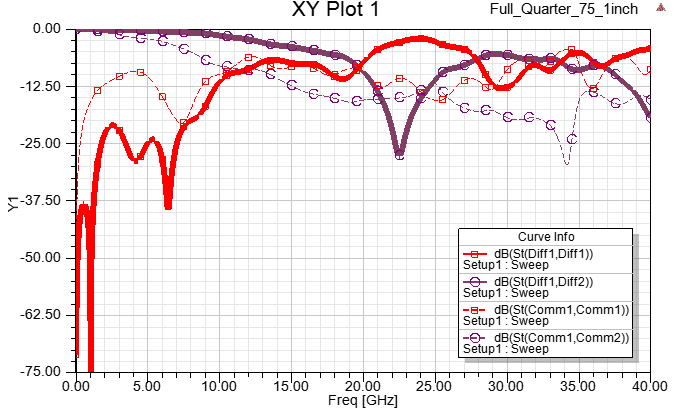
\includegraphics[width=0.8\columnwidth]{./img/PCB/Via_Transition/S_parameter.png}
	\caption{S parameter of via transition in PCB. $r\_anti = 75 mil$. Solid: S11 and S12 of differential mode; dash: S11 and S12 of common mode.}
	\label{fig:pcb_via_tran_S} % label must put at the last
\end{figure}

\begin{figure}[htbp!]
	\centering
	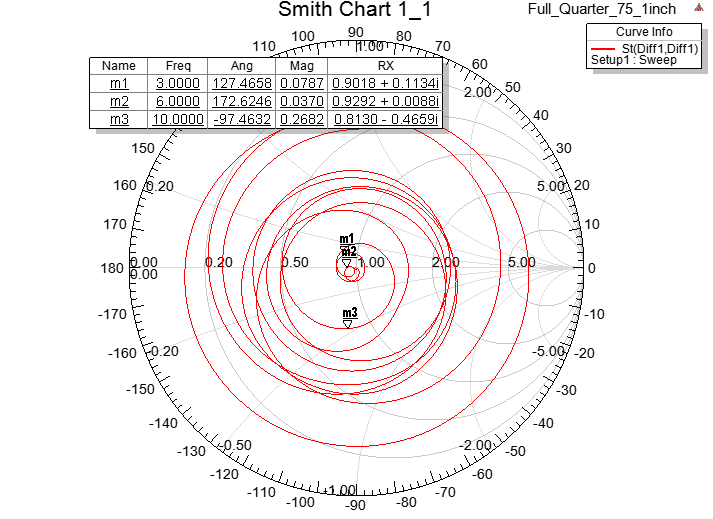
\includegraphics[width=0.8\columnwidth]{./img/PCB/Via_Transition/via_transition_smith.png}
	\caption{Smith chart of $S^{dd}_{11}$ of via transition in PCB.}
	\label{fig:pcb_via_tran_Sdd11_smith} % label must put at the last
\end{figure}

\subsection{Package Traces}
Similar procedure described in \ref{subsec:pcb_traces} can also be applied to the designation of traces on packages. The material properties of substrate used in package is described in Table.~\ref{table:material}.  Fig.~\ref{fig:pkg_trace} and Table.~\ref{table:pkg_trace} shows the design parameters to achieve the desired impedance, and Fig.~\ref{fig:pkg_trace_impedance} shows the impedance of the differential line up to 40 GHz. It shows that the differential impedance is 96$\Omega$ while the common impedance is 25$\Omega$ at 10GHz.

\begin{figure}[htbp!]
	\centering
	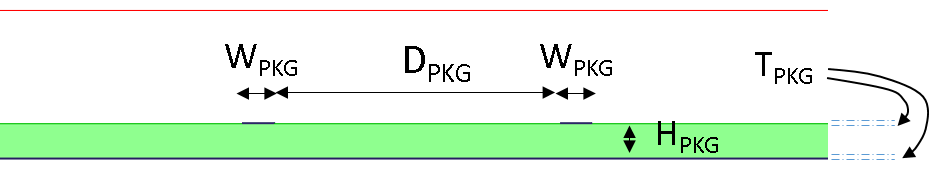
\includegraphics[width=0.8\columnwidth]{./img/PCB/differential_PKG_2D_CrossSection.png}
	\caption{Design parameter of package traces.}
	\label{fig:pkg_trace} % label must put at the last
\end{figure}

\begin{table}[htbp!]
	\renewcommand{\arraystretch}{1.3}	
	\begin{center}
		\begin{tabular}{| c | c | c | c | c | c | c | c |}
			\hline
			Parameters  & Value  & Parameters & Value  & Parameters & Value  & Parameters & Value \\ \hline
			$W_{PKG}$   & 367 um & $D_{PKG}$  & 3.33 mm& $H_{PKG}$  & 400 um & $T_{PKG}$  & 17 um \\
			\hline
		\end{tabular}
	\end{center}
	\label{table:pkg_trace}
	\caption{Design parameter of PCB trace.}
	\vskip0.2in
\end{table}

\begin{figure}[htbp!]
	\centering
	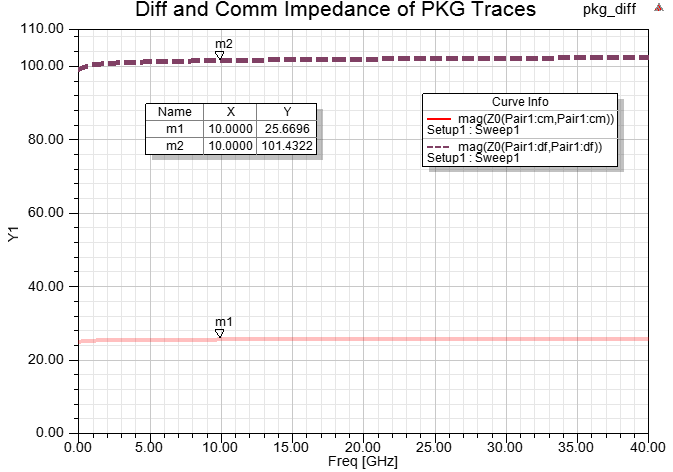
\includegraphics[width=0.8\columnwidth]{./img/PCB/differential_PKG_2D_impedance.png}
	\caption{Differential and common impedance of designated PCB traces. Solid: common mode impedance; dash: differential mode impedance.}
	\label{fig:pkg_trace_impedance} % label must put at the last
\end{figure}



\subsection{Bonding Wire Transition}
\label{sec:bond_wire}
The transition between package and PCB is through using bonding wire. Fig.~\ref{fig:bonding_wire_HFSS} shows the transition structure of bonding wire, and Table.~\ref{table:bonding_wire_parameter} shows the corresponding design parameter. Similar to via transition in PCB described in \ref{subsec:via_tran}, the lumped model shown in \ref{fig:pcb_via_lump_model} also applied here. However, since the bonding wire is a very resistive and inductive, the additional patches were attached at the both side of bonding wire in order to decrease the differential impedance. Same equation in \ref{eq:pcb_via_lump_diff} can also be applied here. 

Fig.~\ref{fig:bonding_wire_S} shows the s parameter of both differential and common mode, and \ref{fig:bonding_wire_S_smith} also shows the $S^{dd}_{11}$ and $S^{dd}_{22}$ on Smith chart. It can be observed that the reflection of differential modes from both ports have 0.1 reflection at 3GHz, whereas half the reflection at 10GHz. The high reflection at high frequency is because adding patches can only be affective at low frequency. In \cite{1IWSPI2S2_FikarS_ScholtzAL_2008_100ghz_bandwidth}, removing ground of both package and PCB will achieve better performance. 

\begin{figure*}[htbp!]
	\centering	
	\begin{minipage}[tb]{\textwidth}
		\centering	
		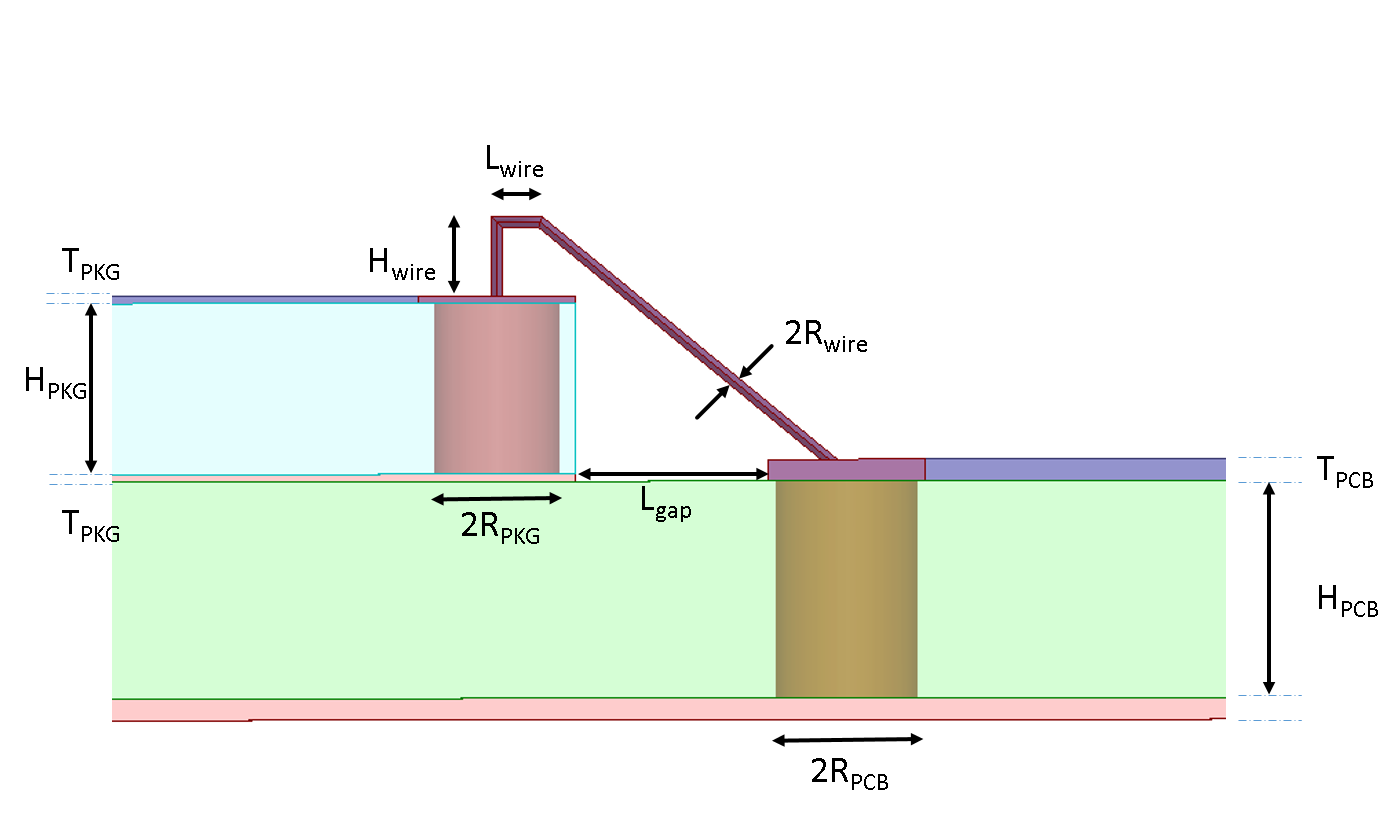
\includegraphics[height=0.4\textheight]{./img/PCB/Bonding_Wire/view-Side.png}
		\subcaption{Side view. The upper left side is package substrate, which is stacked on the PCB substrate. }
	\end{minipage}%
	\vskip0.2in	
	\begin{minipage}[tb]{\textwidth}
		\centering	
		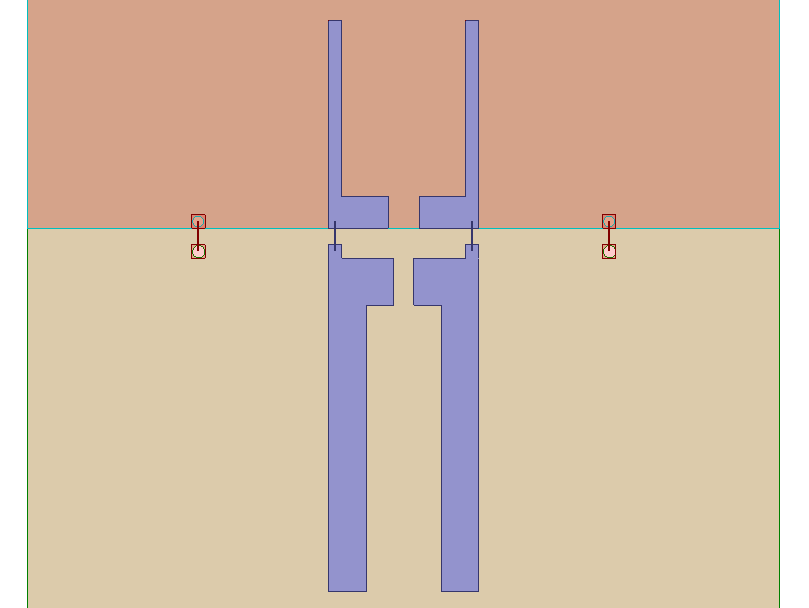
\includegraphics[height=0.4\textheight]{./img/PCB/Bonding_Wire/view-Top.png}
		\subcaption{Top view. The upper side is package substrate. }
	\end{minipage}
	\label{fig:bonding_wire_HFSS}
	\caption{Bonding wire transition simulated in HFSS.}
\end{figure*}

\begin{table}[h]
	\renewcommand{\arraystretch}{1.3}	
	\begin{center}
		\begin{tabular}{| c | c | c | c | c | c | c | c | c | c |}
			\hline
			Parameters  & Value  & Parameters  & Value   & Parameters & Value   & Parameters & Value  \\ \hline
			$G_{PKG}$   & 800 um & $L_{Gap}$   & 450 um  & $R_{PCB}$  & 20 mil  & $R_{PKG}$  & 20 mil \\ \hline
			$H_{Wire}$  & 190 um & $L_{Wire}$  & 100 um  & $R_{Wire}$ & 25 um   & $L_{Gap}$  & 450 um \\ \hline
			$W_{PAD}$   & 367 um & $L_{PAD}$   & 367 um  & $L_{PCB}$  & 10 mm   & $L_{PKG}$  & 6 mm   \\ \hline
			$W_{1}$     & 851 um & $W_{2}$     & 738 um  & $L_{1}$    & 1653 um & $L_{2}$    & 1625 um   \\ \hline
		\end{tabular}
	\end{center}
	\label{table:bonding_wire_parameter}
	\caption{Design parameter of bonding wire transition.}
	\vskip0.2in
\end{table}

\begin{figure}[htbp!]
	\centering
	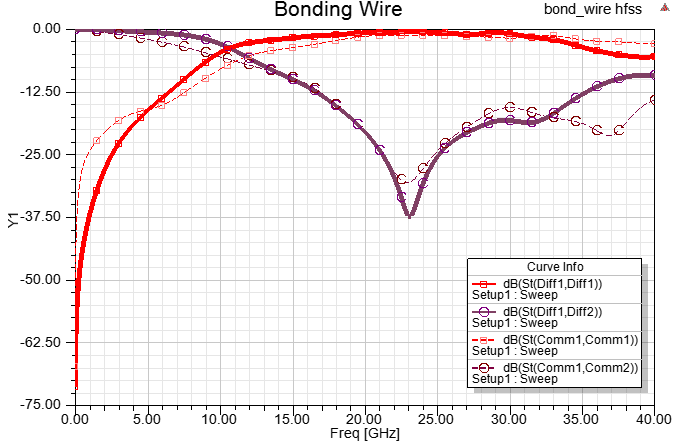
\includegraphics[width=0.8\columnwidth]{./img/PCB/Bonding_Wire/S_param.png}
	\caption{S parameter of bonding wire transition. Solid: S11 and S12 of differential mode; dash: S11 and S12 of common mode.}
	\label{fig:bonding_wire_S} % label must put at the last
\end{figure}

\begin{figure*}[htbp!]
	\centering	
	\begin{minipage}[tb]{0.5\textwidth}
		\centering	
		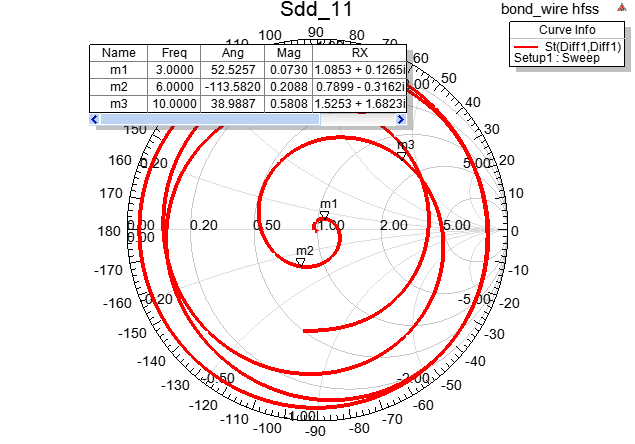
\includegraphics[width=\textwidth]{./img/PCB/Bonding_Wire/Sdd11_smith.png}
		\subcaption{Smith chart of $S^{dd}_{11}$ of bonding wire. }
	\end{minipage}%
	\begin{minipage}[tb]{0.5\textwidth}
		\centering	
		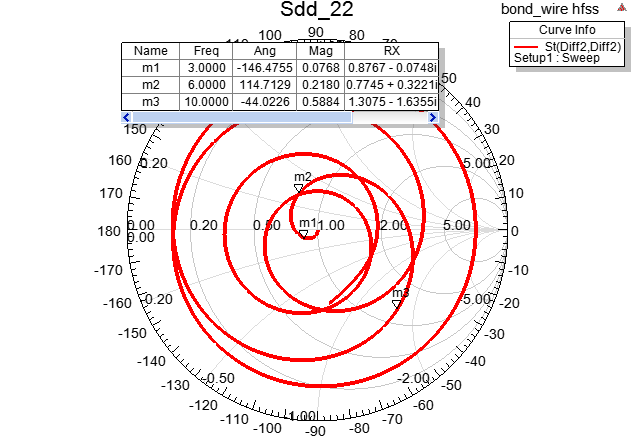
\includegraphics[width=\textwidth]{./img/PCB/Bonding_Wire/Sdd22_smith.png}
		\subcaption{Smith chart of $S^{dd}_{22}$ of bonding wire. }
	\end{minipage}
	\label{fig:bonding_wire_S_smith}
	\caption{Smith chart of Sdd11 and Sdd22 of bonding wire transition.}
\end{figure*}

\begin{figure*}[htbp!]
	\centering	
	\begin{minipage}[b]{0.5\linewidth}
		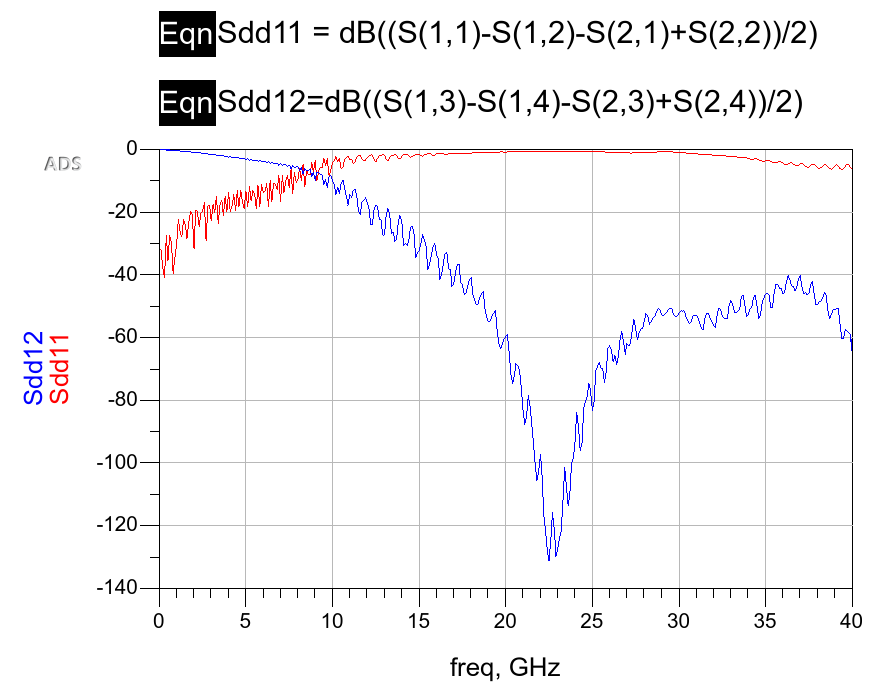
\includegraphics[width=\textwidth]{./img/S-parameter/differential.png}
		\subcaption{Differential Mode.}
	\end{minipage}%
	\begin{minipage}[b]{0.5\linewidth}
		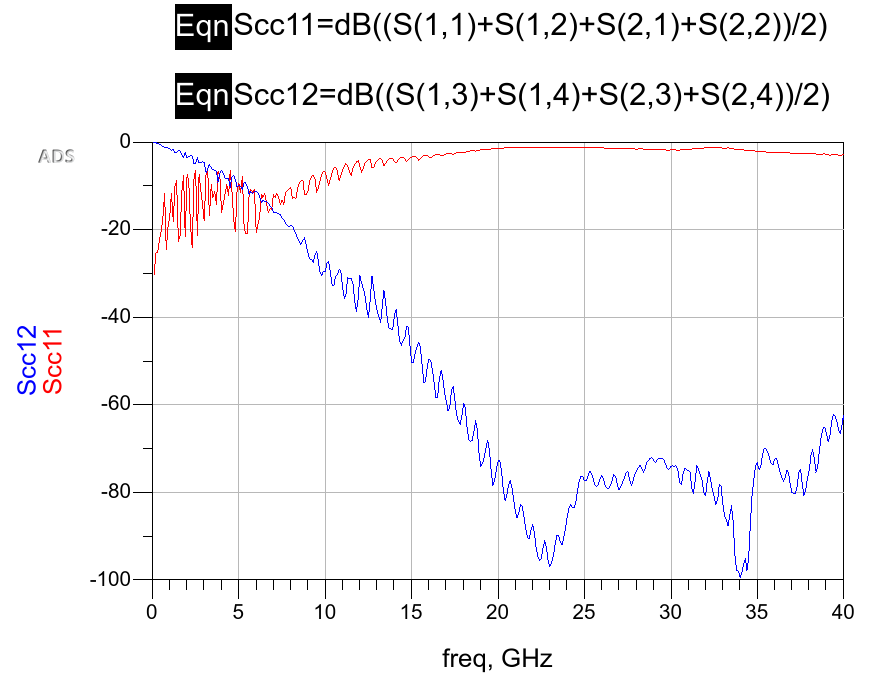
\includegraphics[width=\textwidth]{./img/S-parameter/common.png}
		\subcaption{Common Mode.}
	\end{minipage}
	\begin{minipage}[b]{0.5\linewidth}
		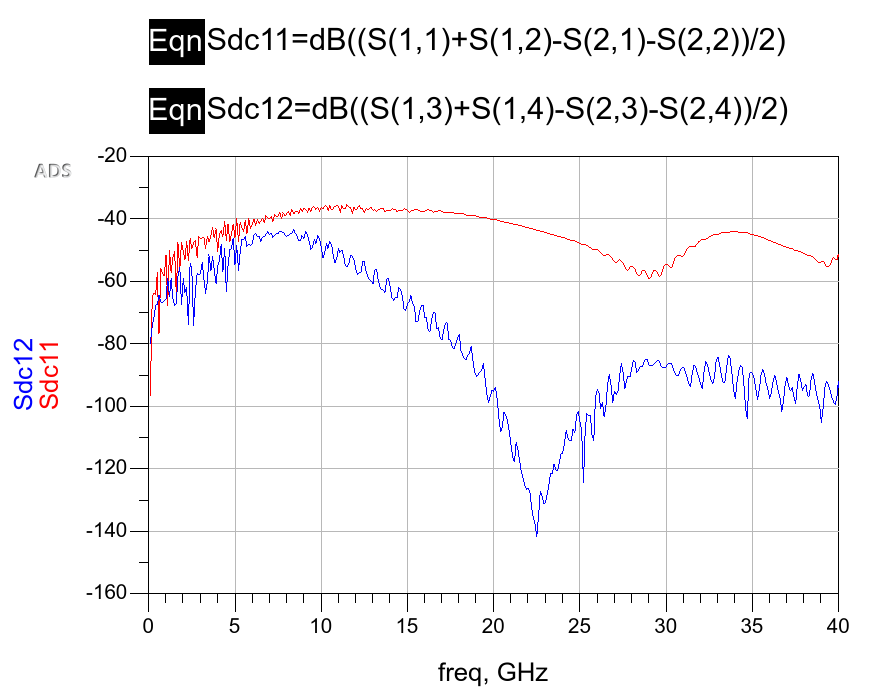
\includegraphics[width=\textwidth]{./img/S-parameter/mixed.png}
		\subcaption{Mixed Mode.}
	\end{minipage}
	\caption{Mixed Mode S-parameter Response.}	
	\label{fig:Mixed Mode S-parameter Response}
\end{figure*}

\subsection{Channel Response}
\begin{figure*}[htbp!]
	\centering	
	\begin{minipage}[tb]{0.5\textwidth}
		\centering	
		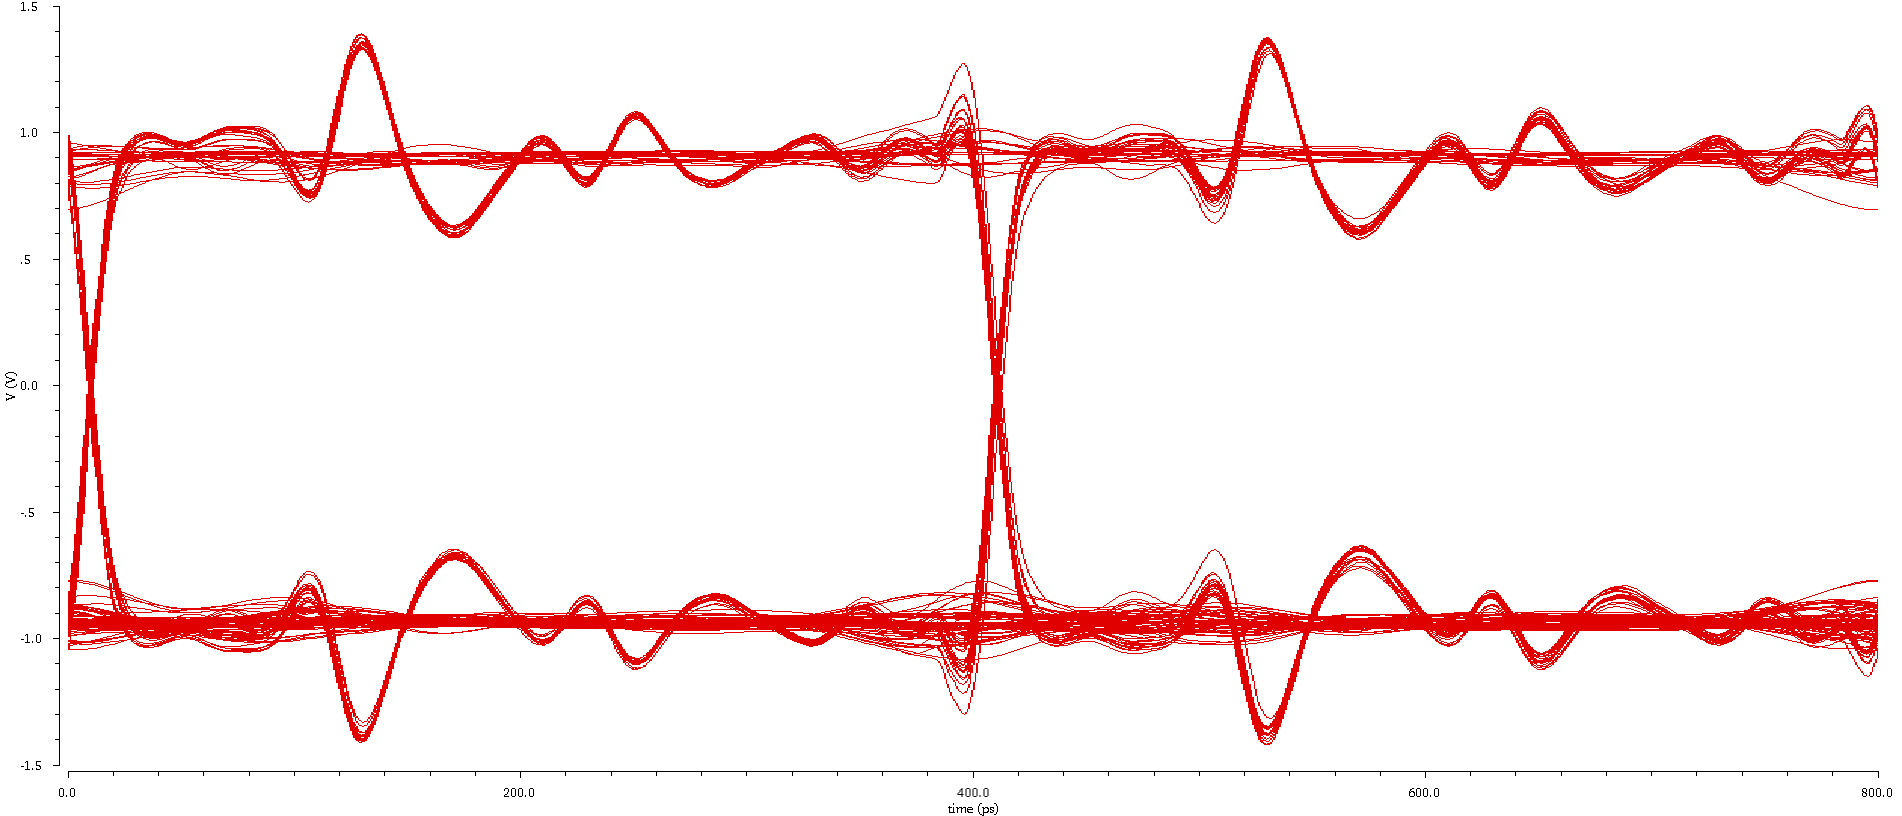
\includegraphics[height=0.15\textheight]{./img/channel_response_eye_diagram/input_differential_eye_3gbp.png}
		\subcaption{3 Gb/s. }
	\end{minipage}%	
	\begin{minipage}[tb]{0.5\textwidth}
		\centering	
		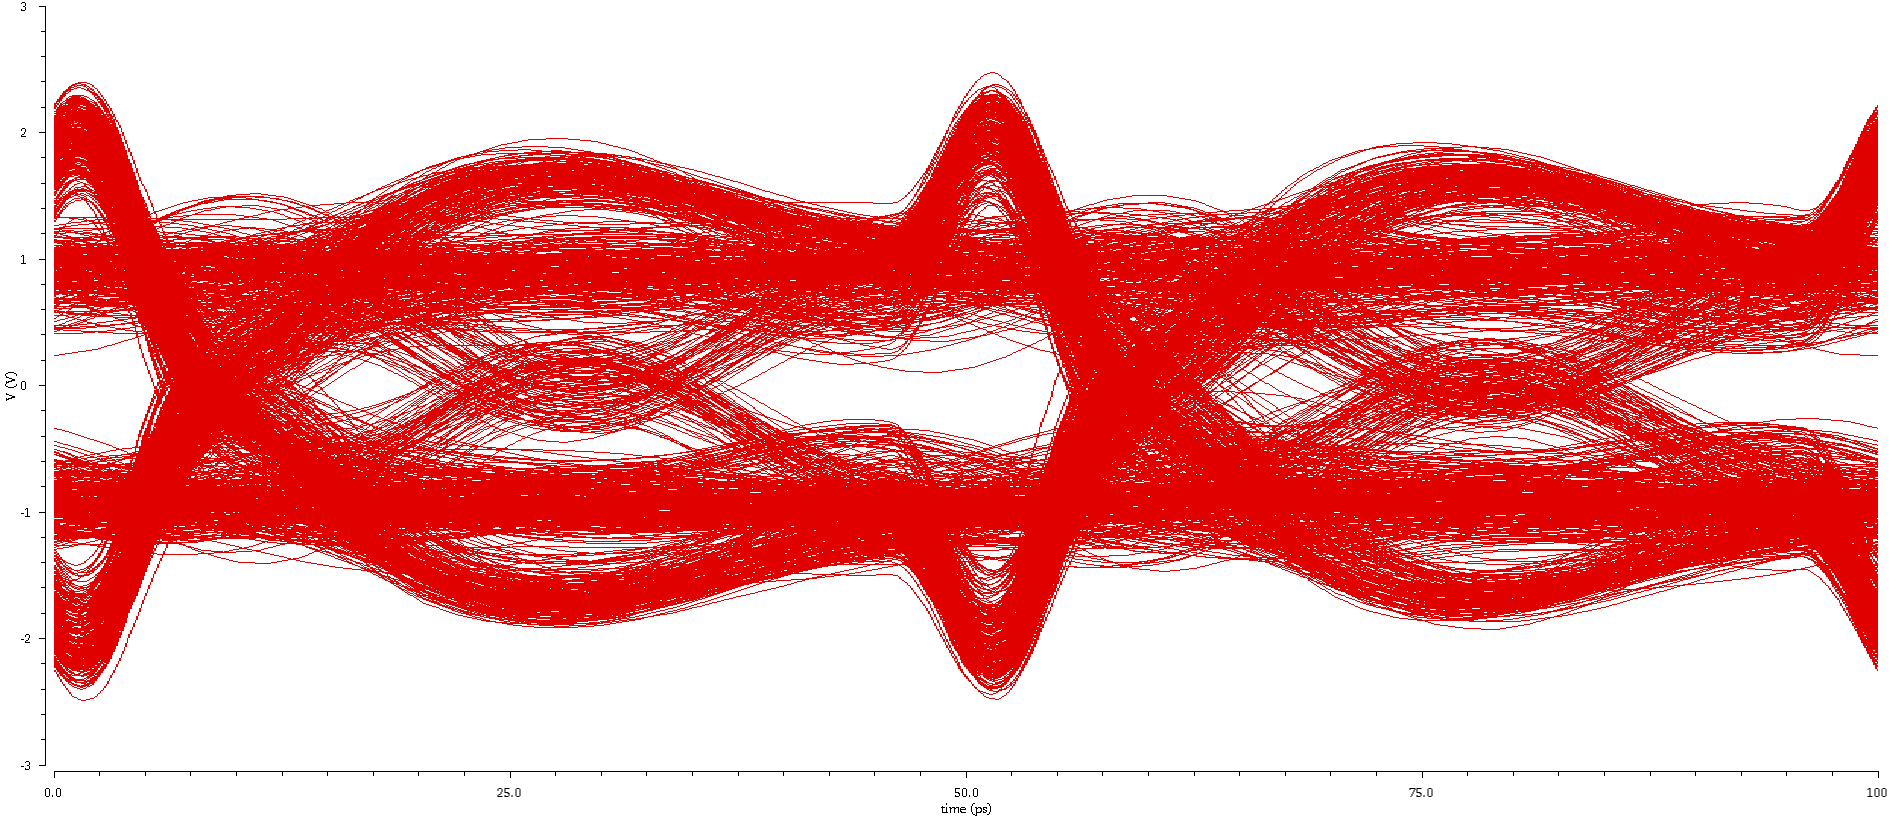
\includegraphics[height=0.15\textheight]{./img/channel_response_eye_diagram/input_differential_eye_20gbp.png}
		\subcaption{20 Gb/s. }
	\end{minipage}
	\caption{Input Eye Diagram.}
	\label{fig:input_differential_eye}
\end{figure*}

\begin{figure*}[htbp!]
	\centering	
	\begin{minipage}[tb]{0.5\textwidth}
		\centering	
		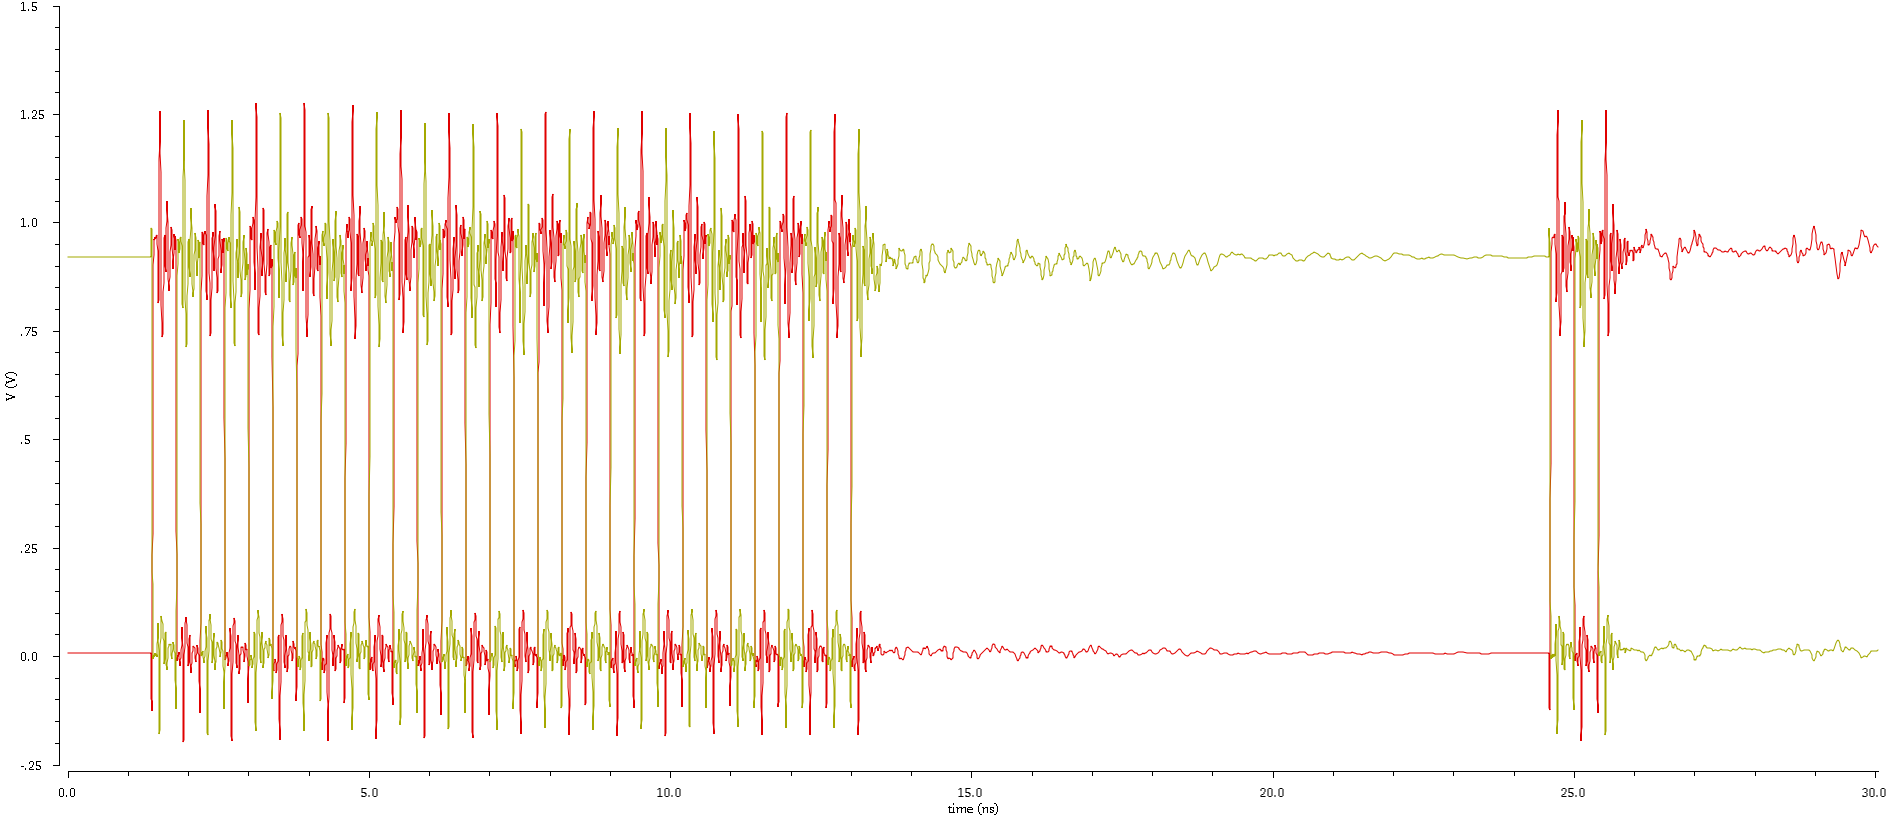
\includegraphics[height=0.15\textheight]{./img/channel_response_eye_diagram/input_transient_response_3gbp.png}
		\subcaption{3 Gb/s. }
	\end{minipage}%	
	\begin{minipage}[tb]{0.5\textwidth}
		\centering	
		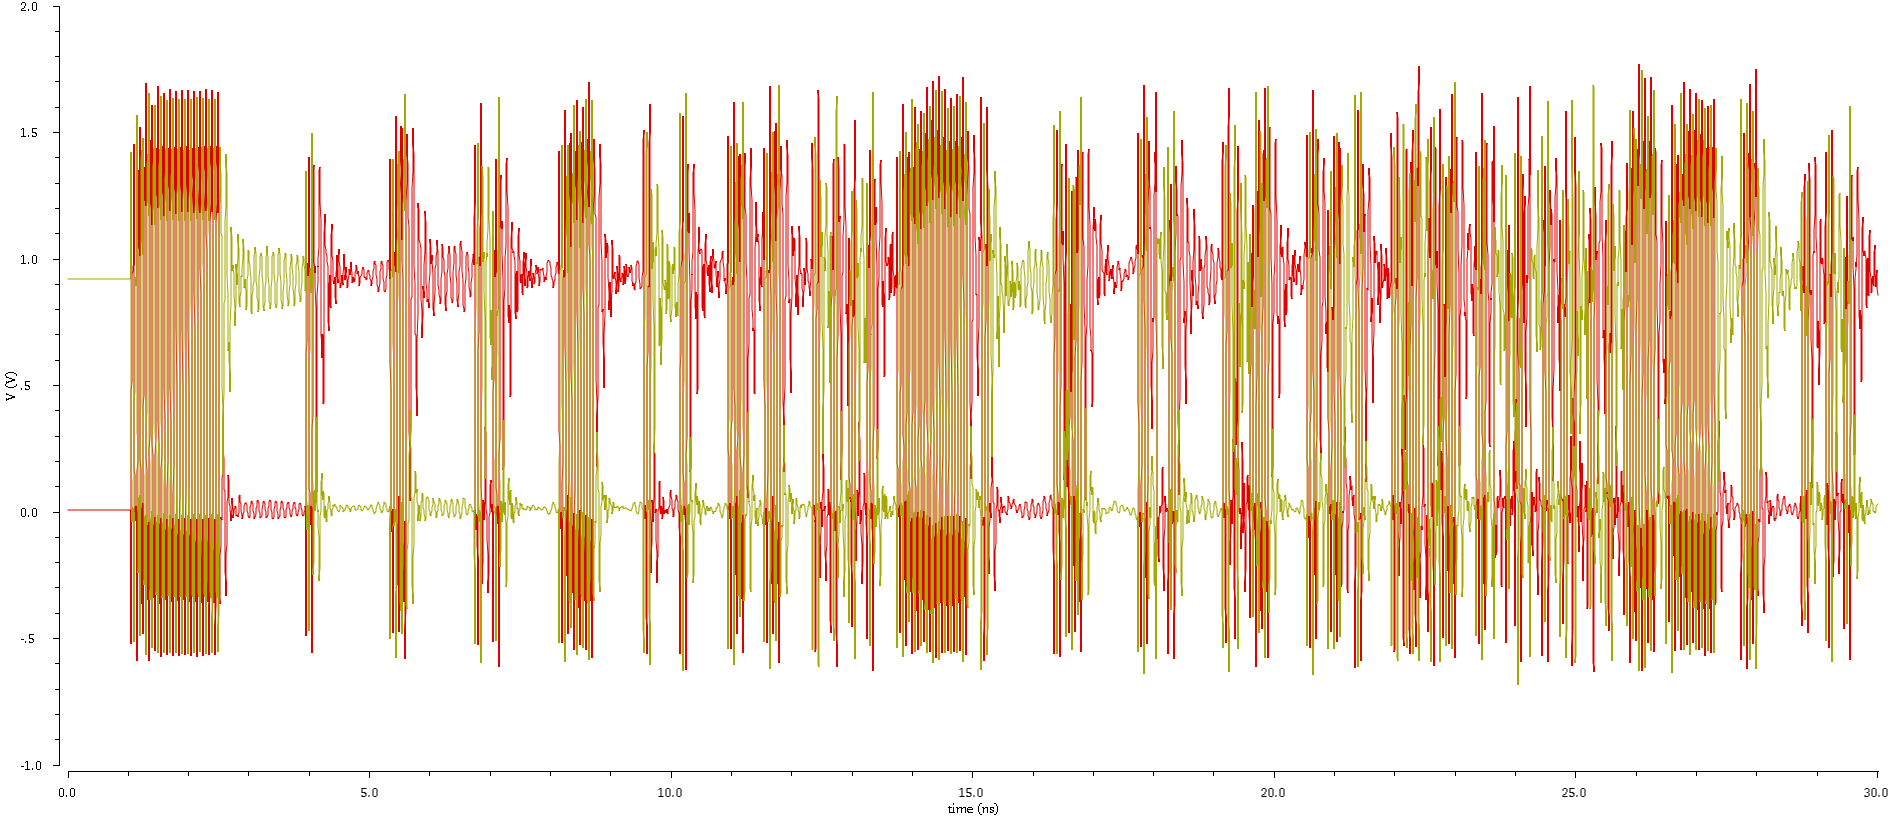
\includegraphics[height=0.15\textheight]{./img/channel_response_eye_diagram/input_transient_response_20gbp.png}
		\subcaption{20 Gb/s. }
	\end{minipage}
	\caption{Input Transient Response.}
	\label{fig:input_transient_response}
\end{figure*}

\begin{figure*}[htbp!]
	\centering	
	\begin{minipage}[tb]{0.5\textwidth}
		\centering	
		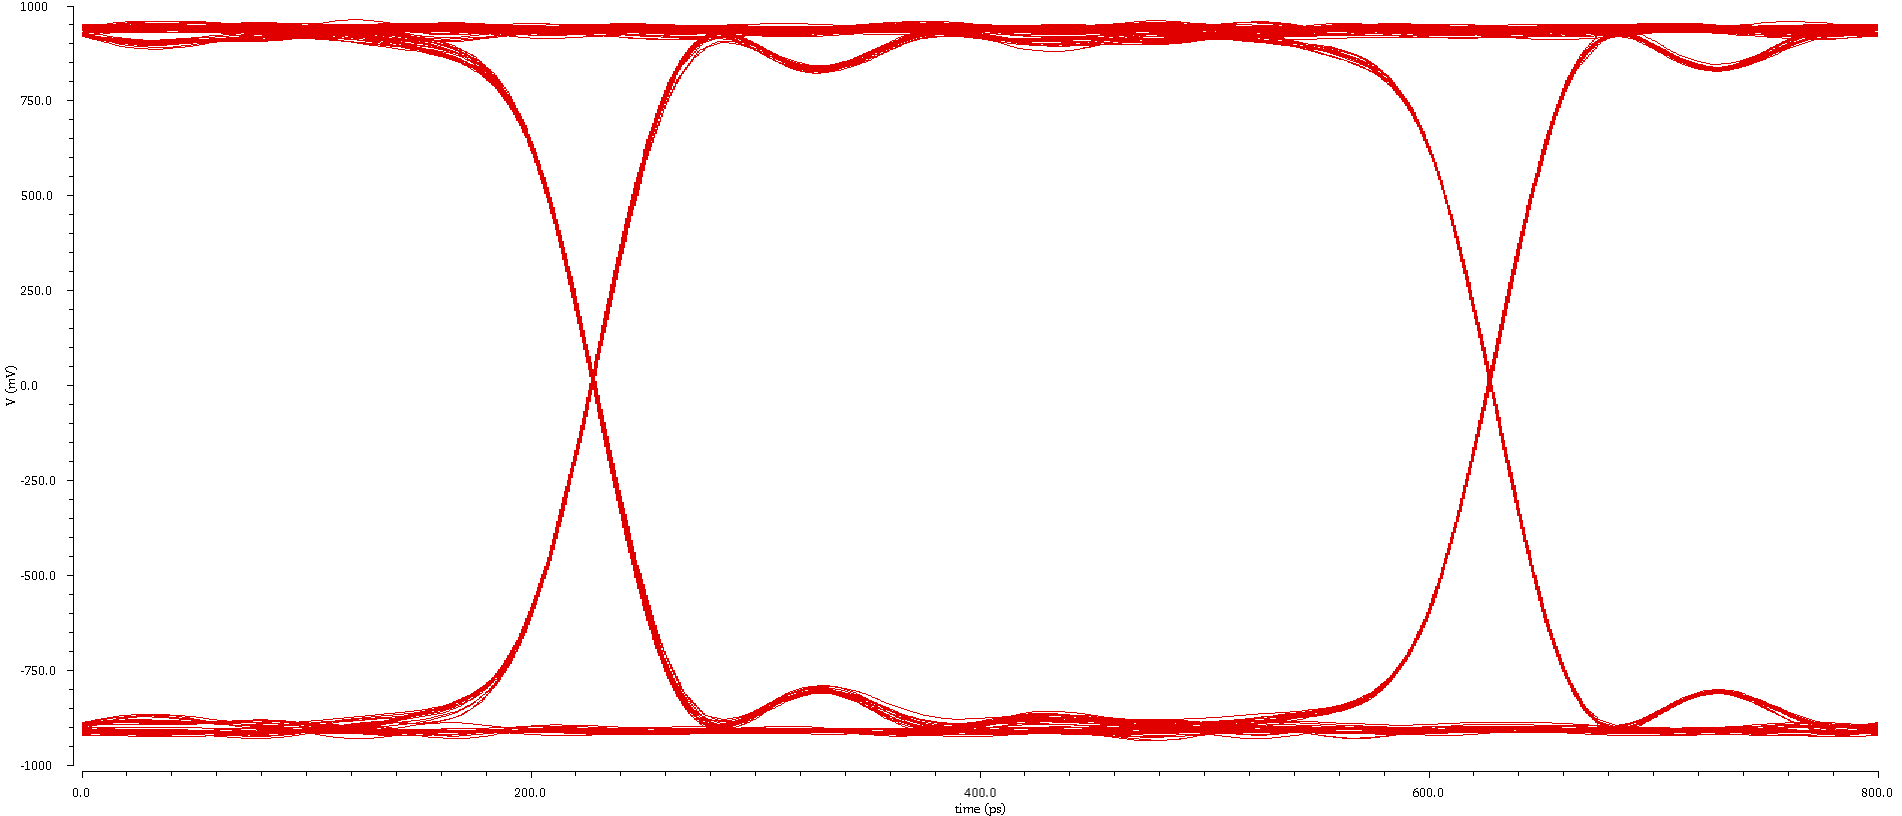
\includegraphics[height=0.15\textheight]{./img/channel_response_eye_diagram/output_differential_eye_3gbp.png}
		\subcaption{3 Gb/s. }
	\end{minipage}%	
	\begin{minipage}[tb]{0.5\textwidth}
		\centering	
		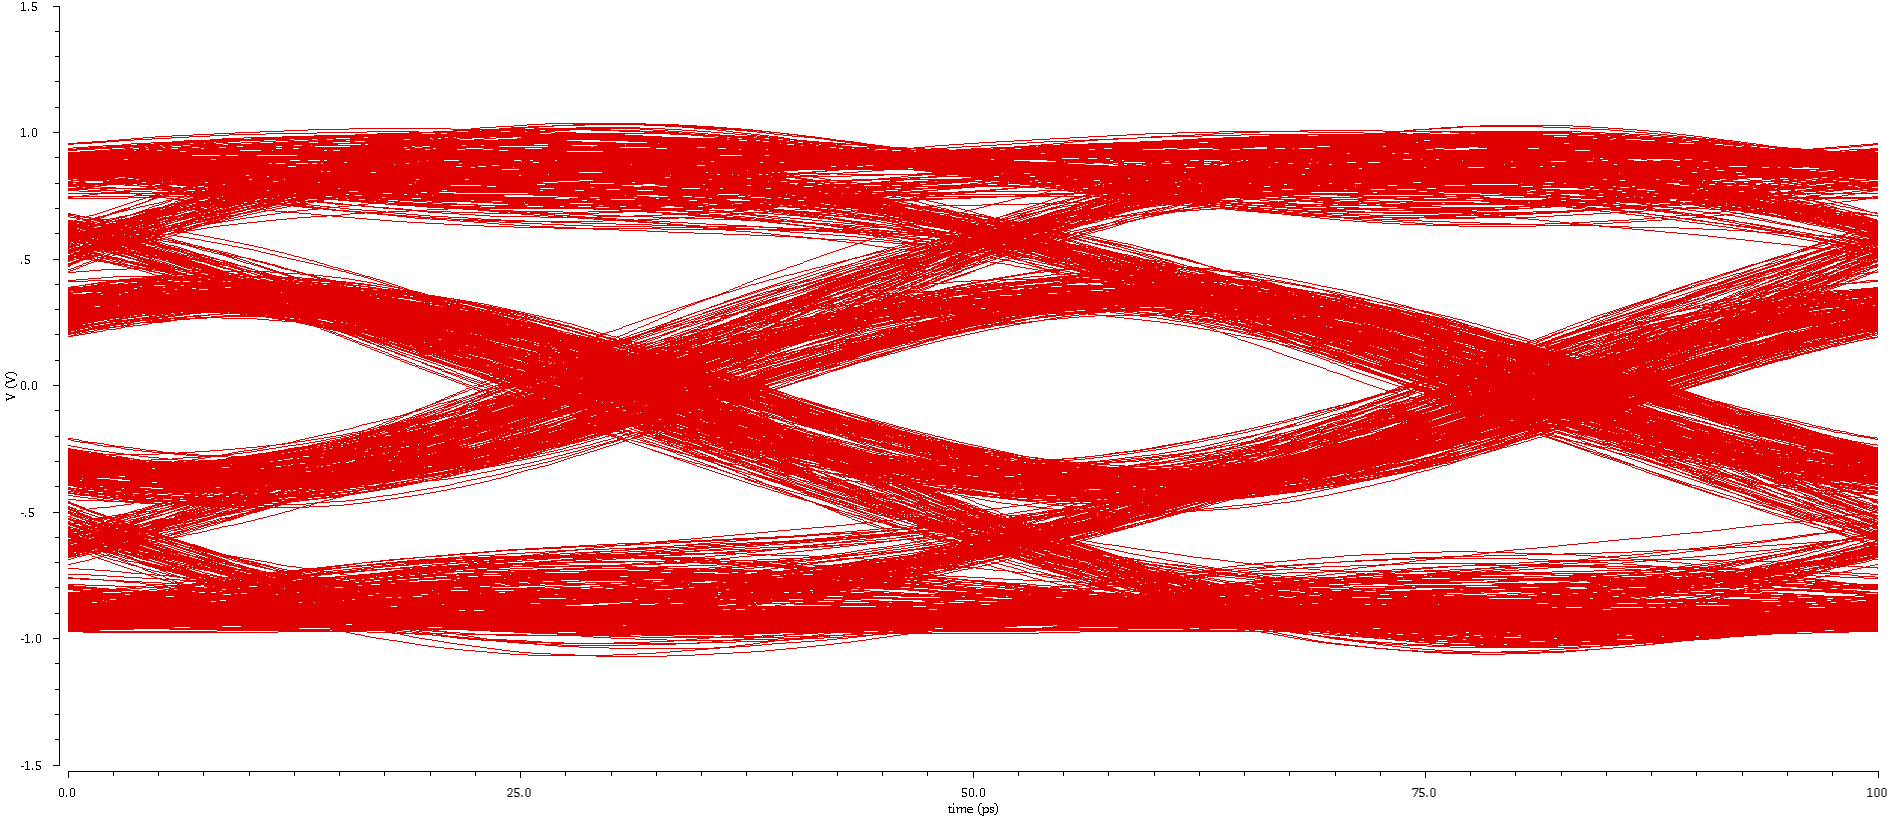
\includegraphics[height=0.15\textheight]{./img/channel_response_eye_diagram/output_differential_eye_20gbp.png}
		\subcaption{20 Gb/s. }
	\end{minipage}
	\caption{Output Eye Diagram.}
	\label{fig:output_differential_eye}
\end{figure*}

\begin{figure*}[htbp!]
	\centering	
	\begin{minipage}[tb]{0.5\textwidth}
		\centering	
		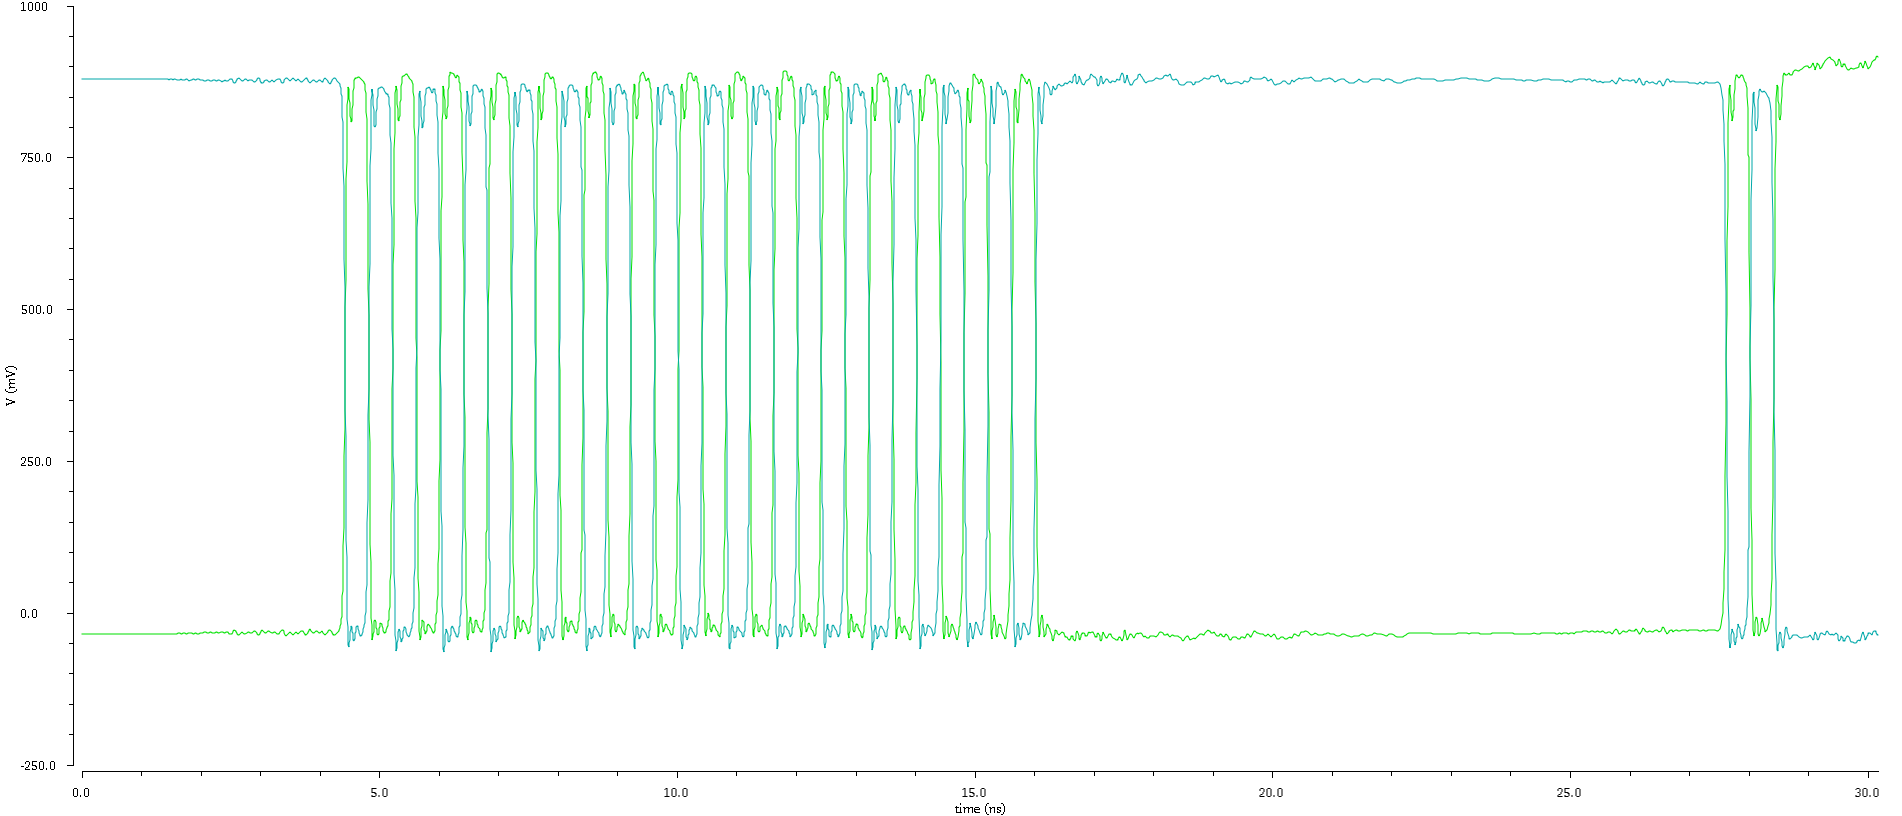
\includegraphics[width=\textwidth]{./img/channel_response_eye_diagram/output_transient_response_3gbp.png}
		\subcaption{3 Gb/s. }
	\end{minipage}%	
	\begin{minipage}[tb]{0.5\textwidth}
		\centering	
		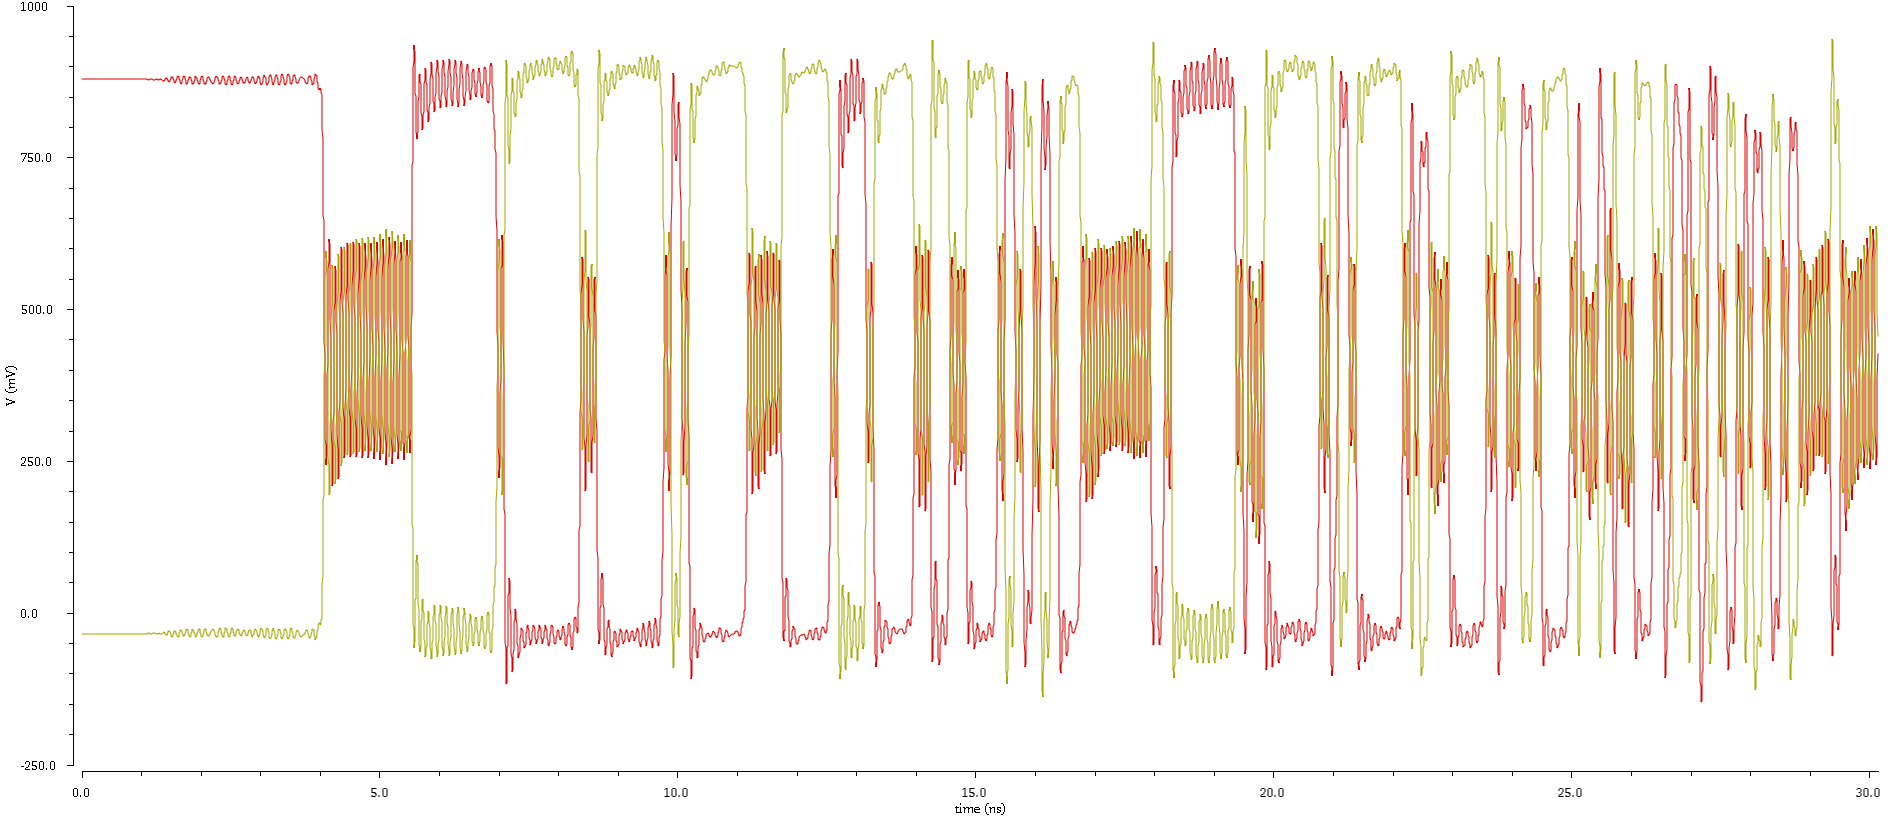
\includegraphics[width=\textwidth]{./img/channel_response_eye_diagram/output_transient_response_20gbp.png}
		\subcaption{20 Gb/s. }
	\end{minipage}
	\caption{Output Transient Response.}
	\label{fig:output_transient_response}
\end{figure*}
\label{subsec:channel_response}
\highlight{Add the entire channel response in time      domain and eye diagram at 3Gbps, and 10Gbps. (With inverter, but without the DFE and FFE)}


\highlight{Add the entire channel response in frequency domain (using ADS), and show the differential / common mode result. }

\section{Feed Forward Equalizer}
\label{sec:FFE}

\begin{figure*}
	\centering	
	\begin{minipage}[tb]{\textwidth}
		\centering	
		\begin{tabular}{|c|c|c|}\hline
			$b_{-2}$ & $b_{-1}$ &  $b_{0}$ \\ \hline 
			0.000 &   -0.001 &    1.016 \\ \hline 
		\end{tabular}
		\label{table:3G_FFE_coeff}
		\subcaption{Coefficient of FFE with 3Gb/s input.}	
	\end{minipage}%
	
	\begin{minipage}[tb]{\textwidth}
		\centering	
		\begin{tabular}{|c|c|c|c|c|c|c|c|c|c|}\hline
			n  &   -2   &   -1   &   0   &    1   &    2   &    3   &    4   &    5   &    6   \\ \hline 
			$V$ & -0.901 & -0.898 & 0.871 & -0.887 & -0.885 & -0.897 & -0.898 & -0.898 & -0.899 \\ \hline
		\end{tabular} 
		\label{table:3G_rxdiff_sample_wo_FFE}
		\subcaption{Sampling signal of received differential w/o FFE.}
	\end{minipage}	
	\begin{minipage}[tb]{\textwidth}
		\centering	
		\begin{tabular}{|c|c|c|c|c|c|c|c|c|c|}\hline
			n  &  -2  &  -1  &  0  &    1   &    2   &    3   &    4   &    5   &    6   \\ \hline 
			$V$ & -0.9 & -0.9 & 0.9 & -0.886 & -0.885 & -0.897 & -0.898 & -0.898 & -0.899 \\ \hline
		\end{tabular}
		\label{table:3G_rxdiff_sample_w__FFE} 
		\subcaption{Sampling signal of received differential with FFE.}
	\end{minipage}
	\caption{FFE Coefficient and Effect of Equalization at 3 Gb/s}
\end{figure*}


\begin{figure*}
	\centering	
	\begin{minipage}[tb]{\textwidth}
		\centering	
		\begin{tabular}{|c|c|c|}\hline
			$b_{-2}$ & $b_{-1}$ &  $b_{0}$ \\ \hline 
			0.146 &   -0.558 &    1.599 \\ \hline
		\end{tabular}
		\label{table:20G_FFE_coeff} 
		\subcaption{Coefficient of FFE with 20Gb/s input.}	
	\end{minipage}%
	
	\begin{minipage}[tb]{\textwidth}
		\centering	
		\begin{tabular}{|c|c|c|c|c|c|c|c|c|c|}\hline
			n  &   -2   &   -1   &   0   &    1   &    2   &    3   &    4   &    5   &    6   \\ \hline 
			$V$ & -0.867 & -0.503 & 0.269 & -0.775 & -0.885 & -0.872 & -0.901 & -0.894 & -0.902 \\ \hline 
		\end{tabular}
		\label{table:20G_rxdiff_sample_wo_FFE}
		\subcaption{Sampling signal of received differential w/o FFE.}
	\end{minipage}	
	\begin{minipage}[tb]{\textwidth}
		\centering	
		\begin{tabular}{|c|c|c|c|c|c|c|c|c|c|}\hline
			n  &   -2   &   -1   &   0   &    1   &    2   &    3   &    4   &    5   &    6   \\ \hline 
			$V$ & -0.898 & -0.898 & 0.901 & -0.705 & -0.892 & -0.854 & -0.906 & -0.889 & -0.905 \\ \hline 
		\end{tabular}
		\label{table:20G_rxdiff_sample_w__FFE} 
		\subcaption{Sampling signal of received differential with FFE.}
	\end{minipage}
	\caption{FFE Coefficient and Effect of Equalization at 20 Gb/s}
\end{figure*}

\begin{figure*}[htbp!]
	\centering	
	\begin{minipage}[tb]{0.5\textwidth}
		\centering	
		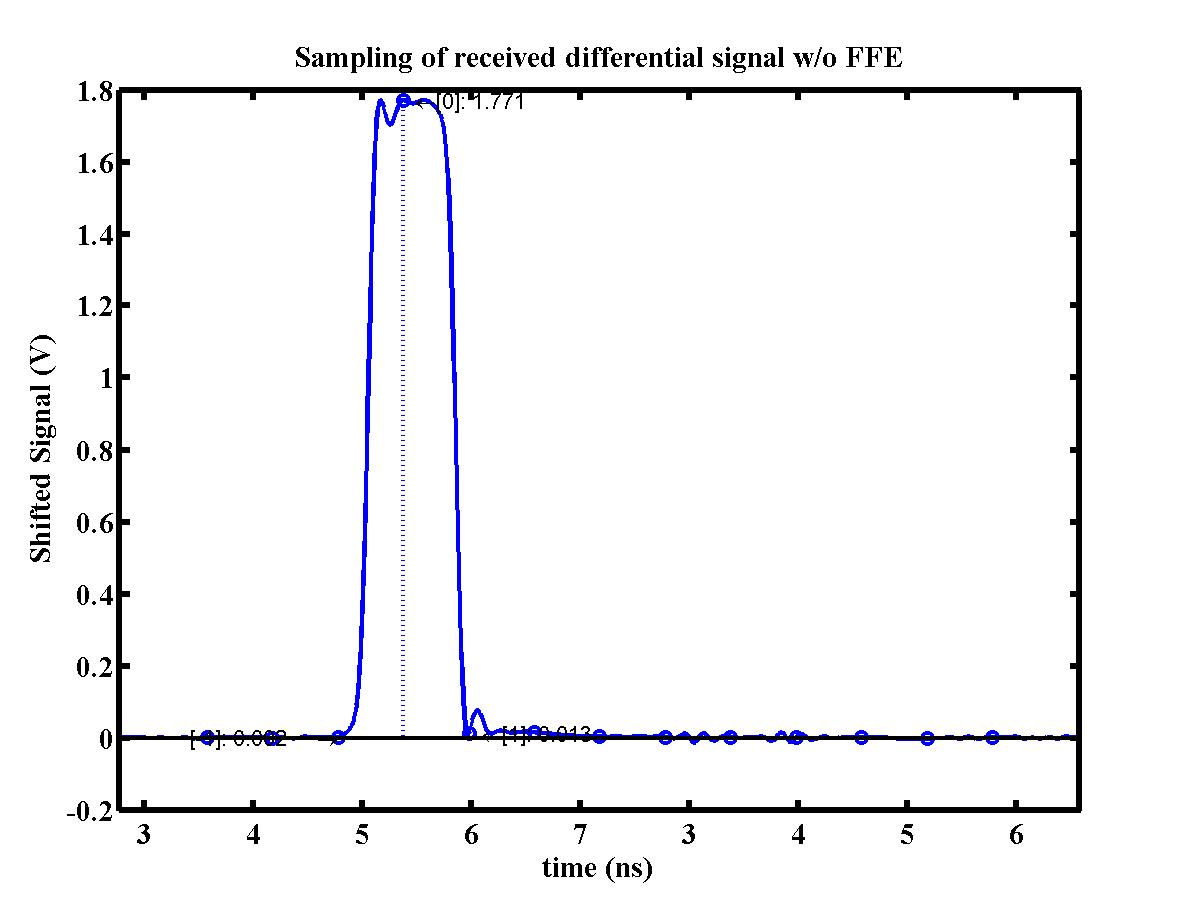
\includegraphics[width=\textwidth]{./img/Verilog/3G/2_sampling.png}
		\subcaption{3 Gb/s. }
	\end{minipage}%	
	\begin{minipage}[tb]{0.5\textwidth}
		\centering	
		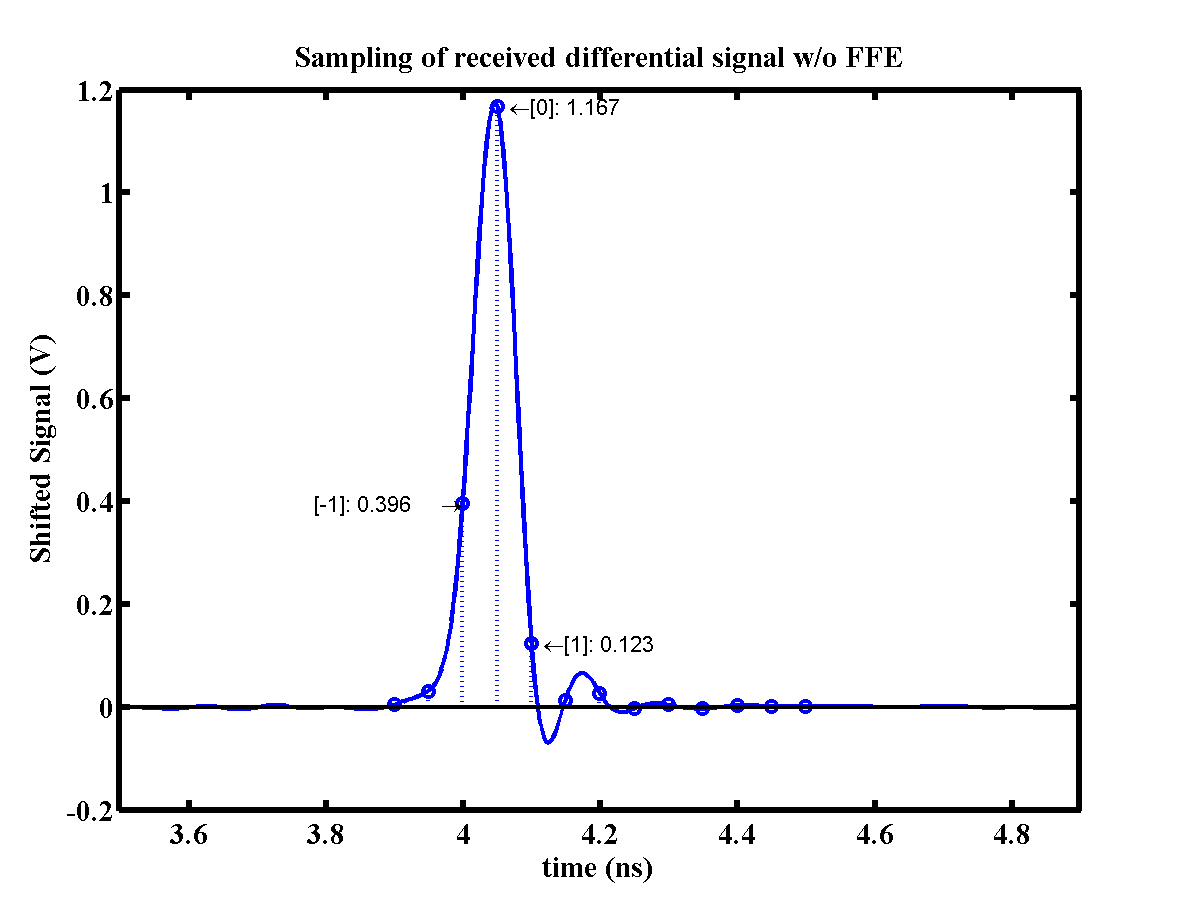
\includegraphics[width=\textwidth]{./img/Verilog/20G/2_sampling.png}
		\subcaption{20 Gb/s. }
	\end{minipage}%	
	\caption{Sampled received differential channel response w/o FFE.}
\end{figure*}

\begin{figure*}[htbp!]
	\centering	
	\begin{minipage}[tb]{0.495\textwidth}
		\centering	
		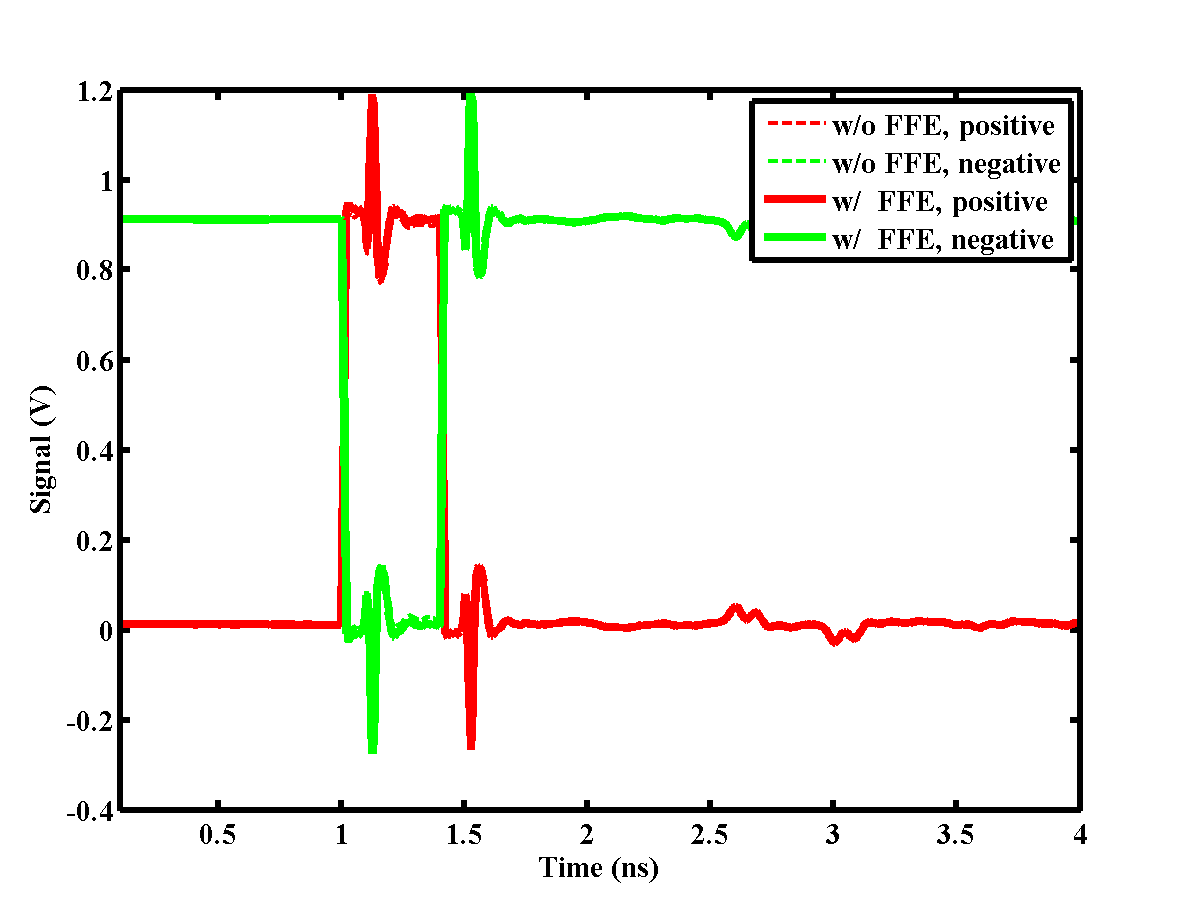
\includegraphics[width=\textwidth]{./img/Verilog/3G/1.png}
		\subcaption{3 Gb/s. }
	\end{minipage}
	\begin{minipage}[tb]{0.495\textwidth}
		\centering	
		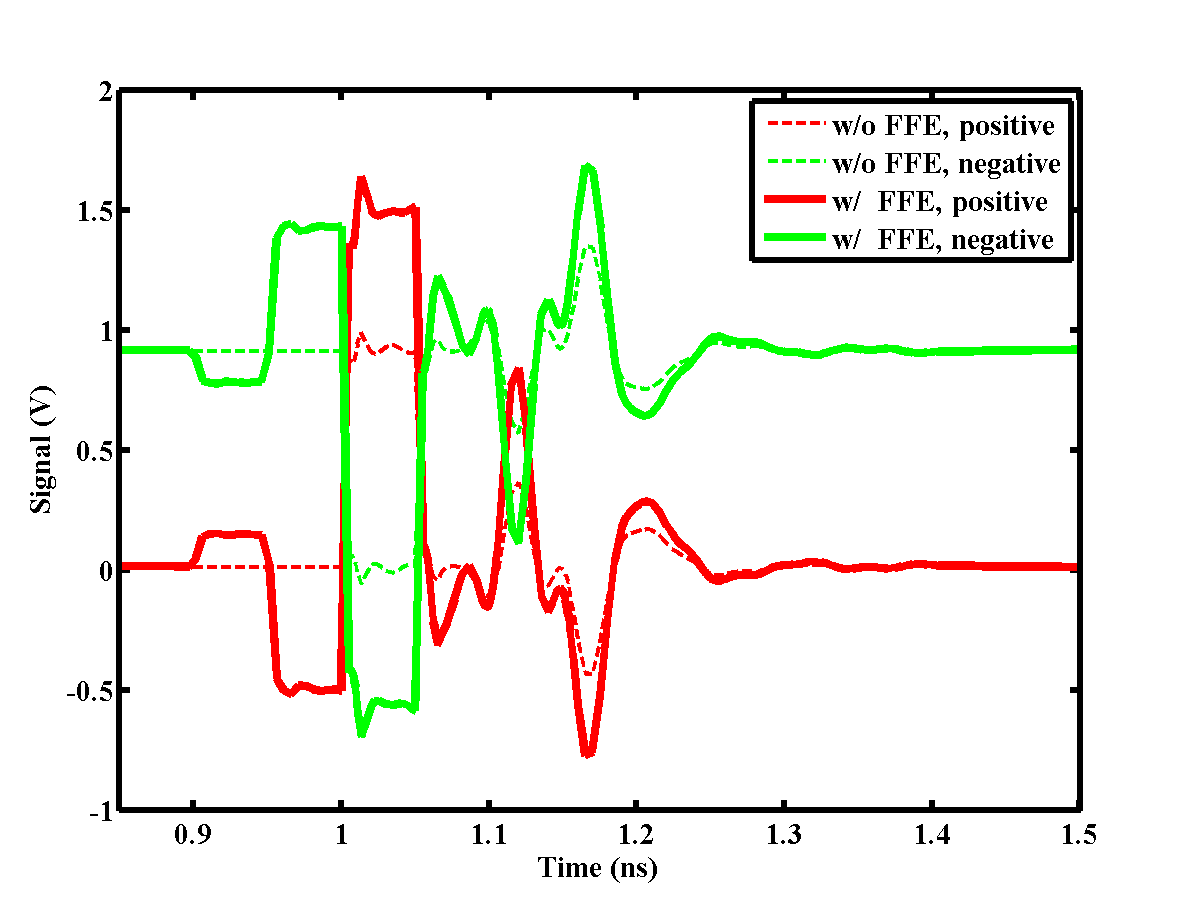
\includegraphics[width=\textwidth]{./img/Verilog/20G/1.png}
		\subcaption{20 Gb/s. }
	\end{minipage}%	
	\caption{Differential signal before channel w/ and w/o FFE.}
\end{figure*}

	
\begin{figure*}[htbp!]	
	\ContinuedFloat
	\begin{minipage}[tb]{0.5\textwidth}
		\centering	
		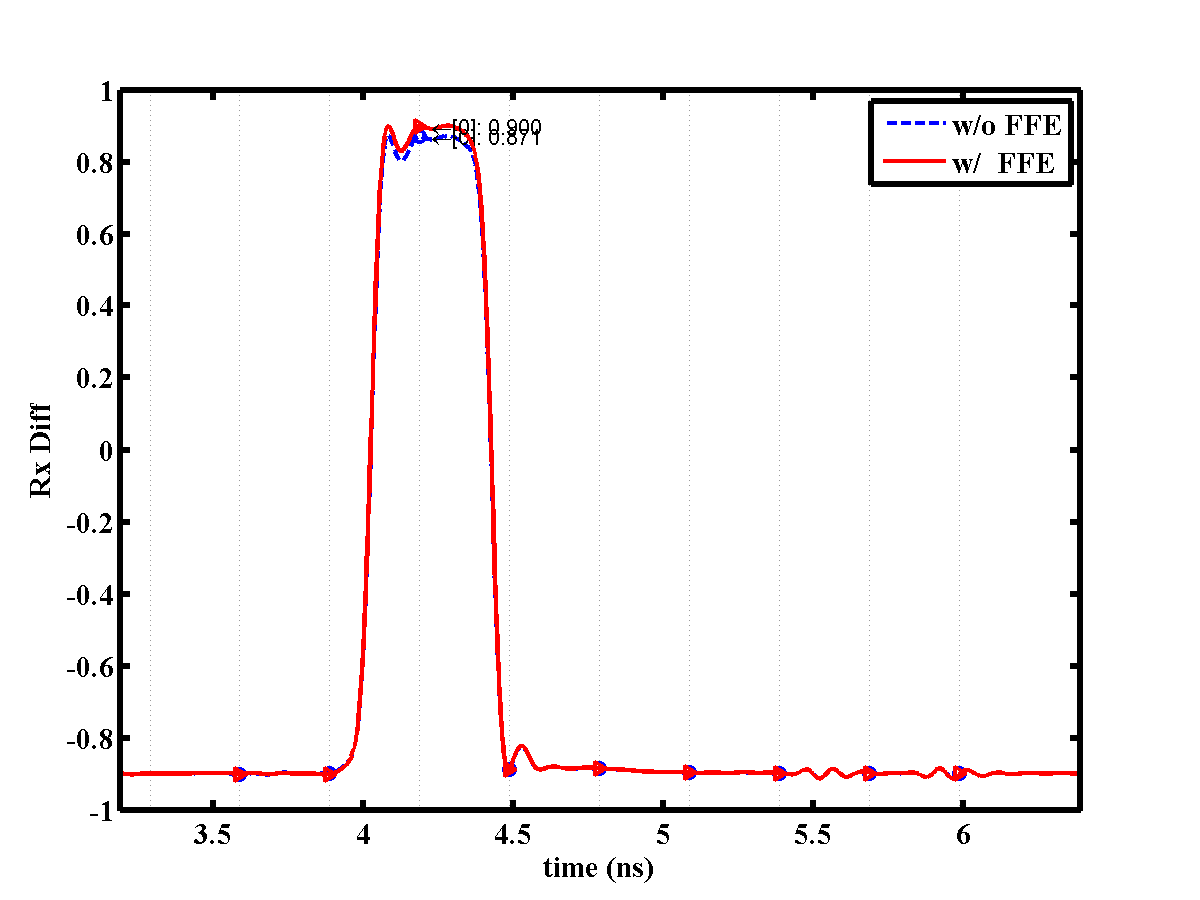
\includegraphics[width=\textwidth]{./img/Verilog/3G/2_diff.png}
		\subcaption{3 Gb/s. }
	\end{minipage}%	
	\begin{minipage}[tb]{0.5\textwidth}
		\centering	
		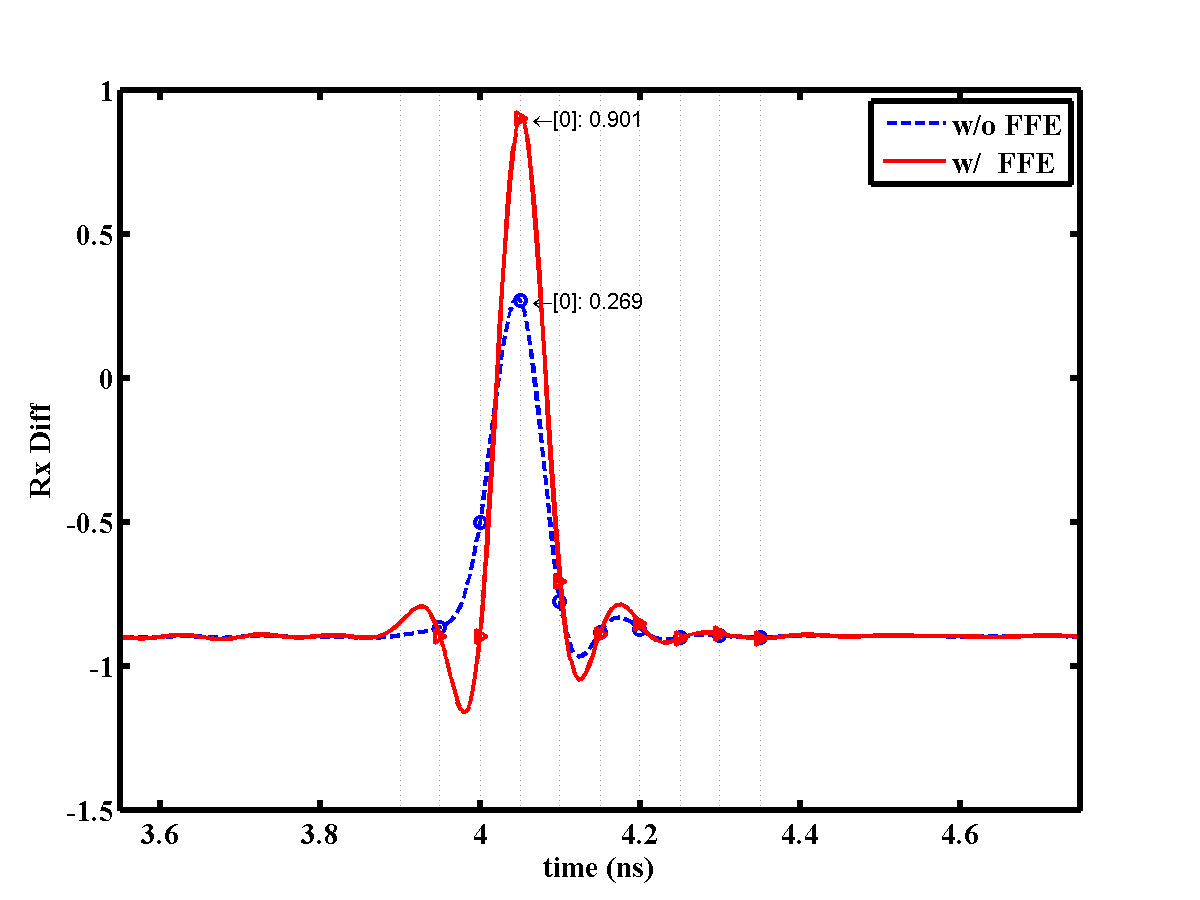
\includegraphics[width=\textwidth]{./img/Verilog/20G/2_diff.png}
		\subcaption{20 Gb/s. }
	\end{minipage}%
	\caption{Received differential channel response w/o or w FFE.}
\end{figure*}

\begin{figure*}[htbp!]	
	\ContinuedFloat
	\begin{minipage}[tb]{0.5\textwidth}
		\centering	
		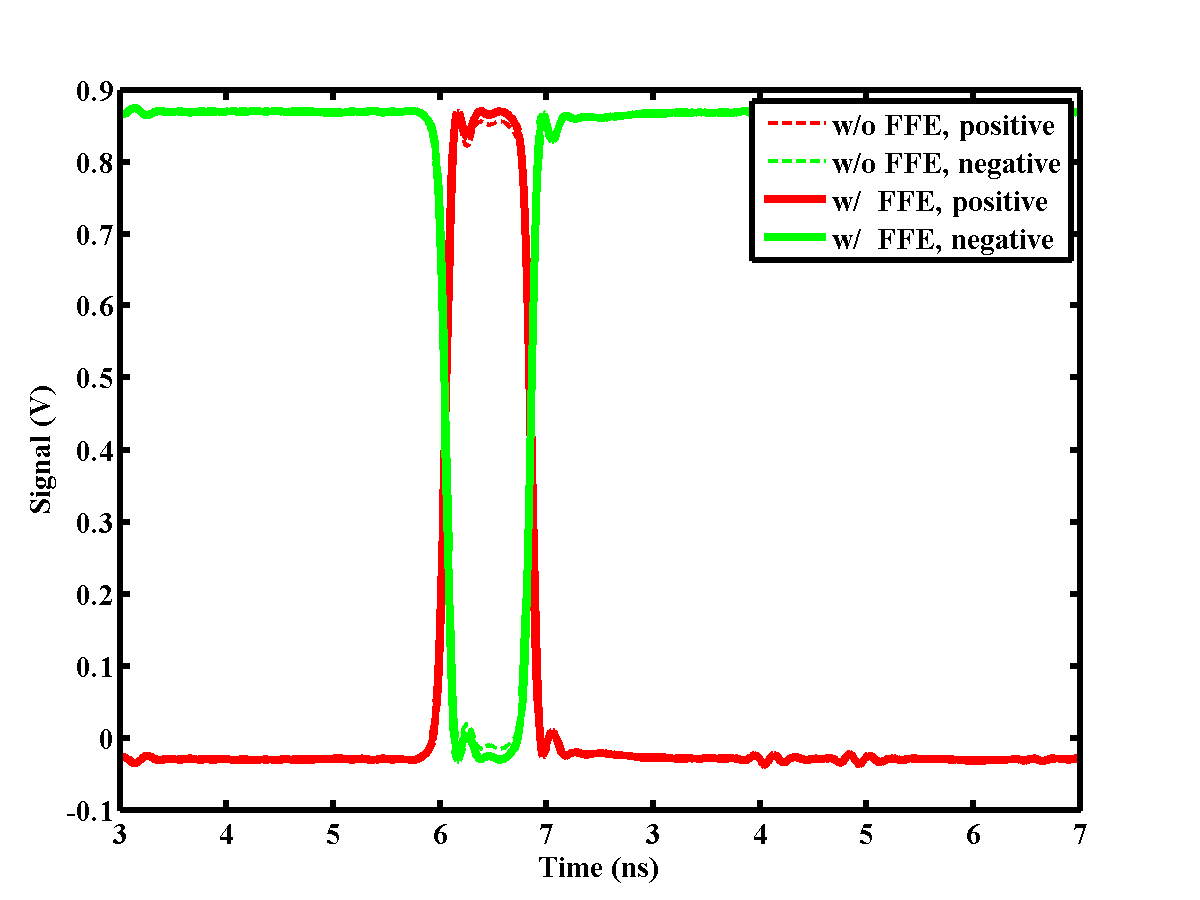
\includegraphics[width=\textwidth]{./img/Verilog/3G/2.png}
		\subcaption{3 Gb/s. }
	\end{minipage}%
	\begin{minipage}[tb]{0.5\textwidth}
		\centering	
		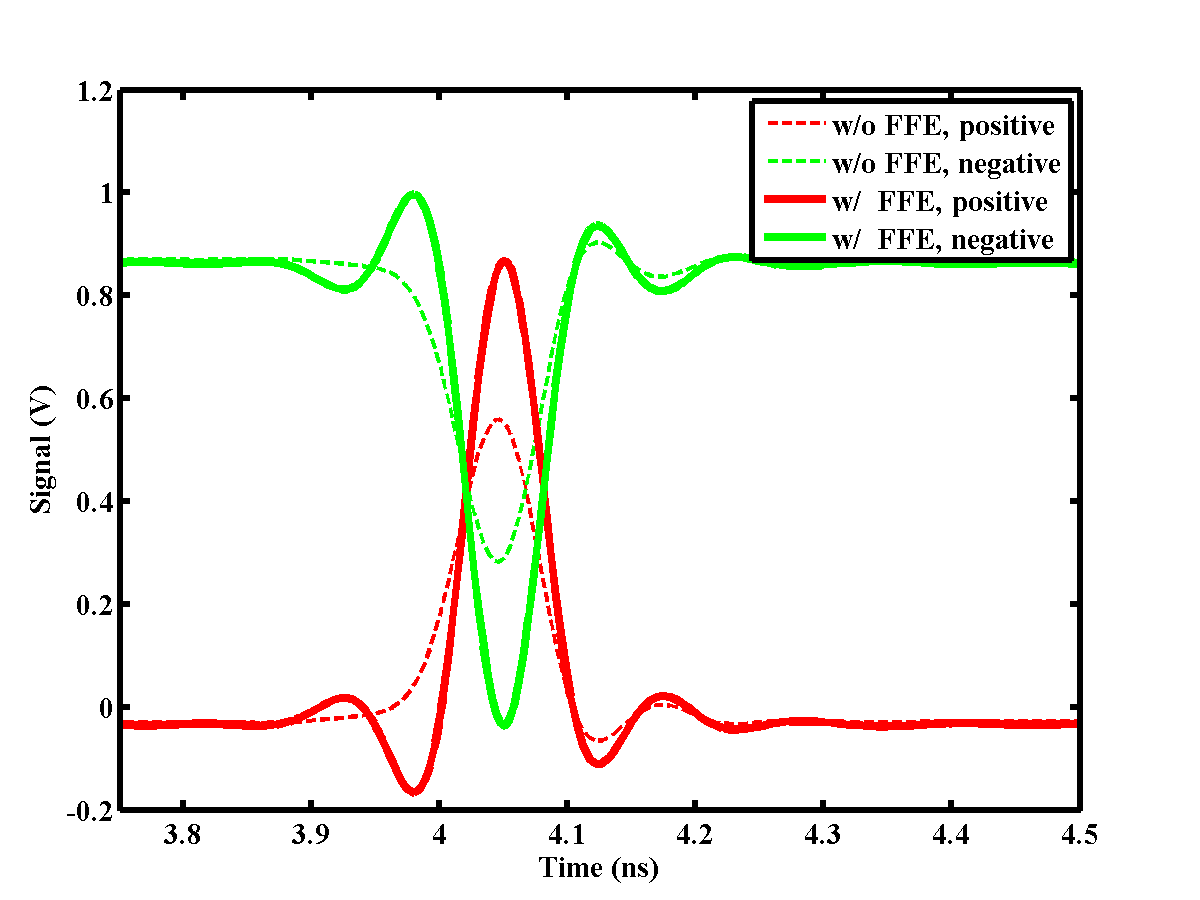
\includegraphics[width=\textwidth]{./img/Verilog/20G/2.png}
		\subcaption{20 Gb/s. }
	\end{minipage}%
	\caption{Differential signal after channel w/ and w/o FFE.}
\end{figure*}


\cphighlight{Add predicted output of FFE}
\cphighlight{TX : Terminal, Diff}
\cphighlight{RX : Terminal, Diff}


\section{Decision Feedback Equalizer}
Decision feedback equalizer (DFE) is a finite impulse response (FIR) filter based feedback scheme that reduces intersymbol Interference (ISI). The DFE consists of a slicer (Decision unit) and a FIR filter. The slicer makes symbol decisions and determine whether the FIR filter should be used to reduce the postcursors. By analyzing the input differential signal, we can predict the magnitude of postcursors and substract it ahead. Postcursors can then be reduced by making filter tap coefficients equal to postcursor magnitude but with an opposite sign.  
%
\begin{equation}
c_i = V_d^{Rx}[n] - V_d^{Rx}[\infty], n=1,2,...,5,
\label{eq:DFE_tap_design_formula}
\end{equation}
%
<<<<<<< HEAD
where $V_d^{Rx}[n]$ is the n-th sampling of received differential signal with FFE enabled. Since there might be DC locc in the channel, the base level, or the steady state of the differential signal may not be exactly -0.9V and thus $V_d^{Rx}[\infty]$, the steady state of the received differential signal must be substracted before using \ref{eq:DFE_tap_design_formula}. The sampling rate of DFE is the same to the system clock rate. When integrate the DFE unit into the entire channel, appropriate delay time needs to be added to ensure correct functioning of the DFE. In our case, we set our delay time to be 4.2 ns. 


\begin{figure*}
	\centering	
	\begin{minipage}[tb]{\textwidth}
		\centering	
		\begin{tabular}{|c|c|c|c|c|}\hline
			$c_{1}$ &  $c_{2}$ &  $c_{3}$ &  $c_{4}$ &  $c_{5}$ \\ \hline 
			0.014 &    0.015 &    0.004 &    0.003 &    0.002 \\ \hline 
		\end{tabular}
		\label{table:3G_DFE_coeff}
		\subcaption{Coefficient of DFE with 3Gb/s input.}	
	\end{minipage}%
	
	\begin{minipage}[tb]{\textwidth}
		\centering	
		\begin{tabular}{|c|c|c|c|c|c|c|c|c|c|}\hline
			n  &  -2  &  -1  &  0  &    1   &    2   &    3   &    4   &    5   &    6   \\ \hline 
			$V$ & -0.9 & -0.9 & 0.9 & -0.886 & -0.885 & -0.897 & -0.898 & -0.898 & -0.899 \\ \hline 
		\end{tabular}
		\label{table:3G_rxdiff_sample_wo_DFE}
		\subcaption{Sampling signal of received differential w/o DFE.}
	\end{minipage}	
	\begin{minipage}[tb]{\textwidth}
		\centering	
		\begin{tabular}{|c|c|c|c|c|c|c|c|c|c|}\hline
			n  &  -2  &  -1  &  0  &   1  &   2  &   3  &   4  &   5  &    6   \\ \hline 
			$V$ & -0.9 & -0.9 & 0.9 & -0.9 & -0.9 & -0.9 & -0.9 & -0.9 & -0.899 \\ \hline 
		\end{tabular}
		\label{table:3G_rxdiff_sample_w__DFE} 
		\subcaption{Sampling signal of received differential with DFE.}
	\end{minipage}
	\caption{DFE Coefficient and Effect of Equalization at 3 Gb/s}
\end{figure*}

\begin{figure*}
	\centering	
	\begin{minipage}[tb]{\textwidth}
		\centering	
		\begin{tabular}{|c|c|c|c|c|}\hline
			$c_{1}$ &  $c_{2}$ &  $c_{3}$ &  $c_{4}$ &  $c_{5}$ \\ \hline 
			0.194 &    0.007 &    0.046 &   -0.007 &    0.011 \\ \hline 
		\end{tabular}
		\label{table:20G_DFE_coeff} 
		\subcaption{Coefficient of DFE with 20Gb/s input.}	
	\end{minipage}%
	
	\begin{minipage}[tb]{\textwidth}
		\centering	
		\begin{tabular}{|c|c|c|c|c|c|c|c|c|c|}\hline
			n  &   -2   &   -1   &   0   &    1   &    2   &    3   &    4   &    5   &    6   \\ \hline 
			$V$ & -0.898 & -0.898 & 0.901 & -0.705 & -0.892 & -0.854 & -0.906 & -0.889 & -0.905 \\ \hline 
		\end{tabular}
		\label{table:20G_rxdiff_sample_wo_DFE}
		\subcaption{Sampling signal of received differential w/o DFE.}
	\end{minipage}	
	\begin{minipage}[tb]{\textwidth}
		\centering	
		\begin{tabular}{|c|c|c|c|c|c|c|c|c|c|}\hline
			n  &   -2   &   -1   &   0   &    1   &    2   &    3   &    4   &    5   &    6   \\ \hline 
			$V$ & -0.898 & -0.898 & 0.901 & -0.899 & -0.899 & -0.899 & -0.899 & -0.899 & -0.905 \\ \hline 
		\end{tabular}
		\label{table:20G_rxdiff_sample_w__DFE} 
		\subcaption{Sampling signal of received differential with DFE.}
	\end{minipage}
	\caption{DFE Coefficient and Effect of Equalization at 20 Gb/s}
\end{figure*}

where $V_d^{Rx}[n]$ is the n-th sampling of received differential signal with FFE enabled. Since there might be DC locc in the channel, the base level, or the steady state of the differential signal may not be exactly -0.9V and thus $V_d^{Rx}[\infty]$, the steady state of the received differential signal must be substracted before using \ref{eq:DFE_tap_design_formula}. The sampling rate of DFE is the same to the system clock rate.

However, there are several different delay scheme of DFE. The traditional delay scheme is one delay, as shown in left figure of \ref{fig:dfe_delay_scheme}. 

\cphighlight{This is proposed in  Another }

\begin{figure}[htbp!]
	\centering
	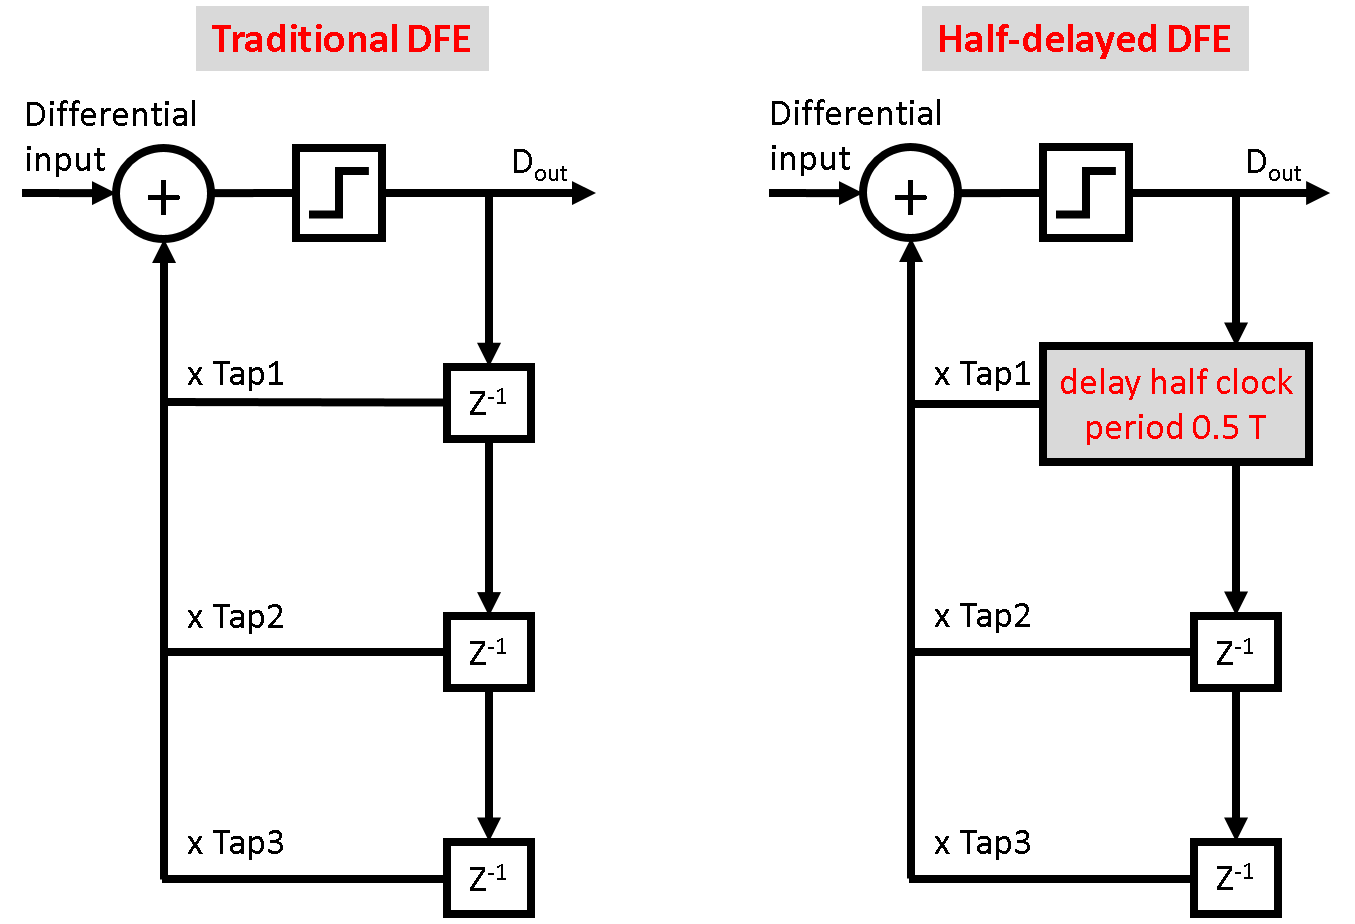
\includegraphics[width=0.8\columnwidth]{./img/Verilog/half-delayed_DFE_comparison.png}
	\caption{Different delay scheme of DFE.}
	\label{fig:dfe_delay_scheme} % label must put at the last
\end{figure}


\cphighlight{Add predicted output of FFE + DFE}
\cphighlight{RX : Terminal, Diff}
\cphighlight{RXe: Terminal, Diff}

\section{Differential Amplifier}
\label{sec:diff_Op}

\section{Result}
\label{sec:result}

\begin{figure*}[htbp!]
	\captionsetup[subfigure]{justification=centering}
	\begin{minipage}[tb]{0.5\textwidth}
		\centering	
		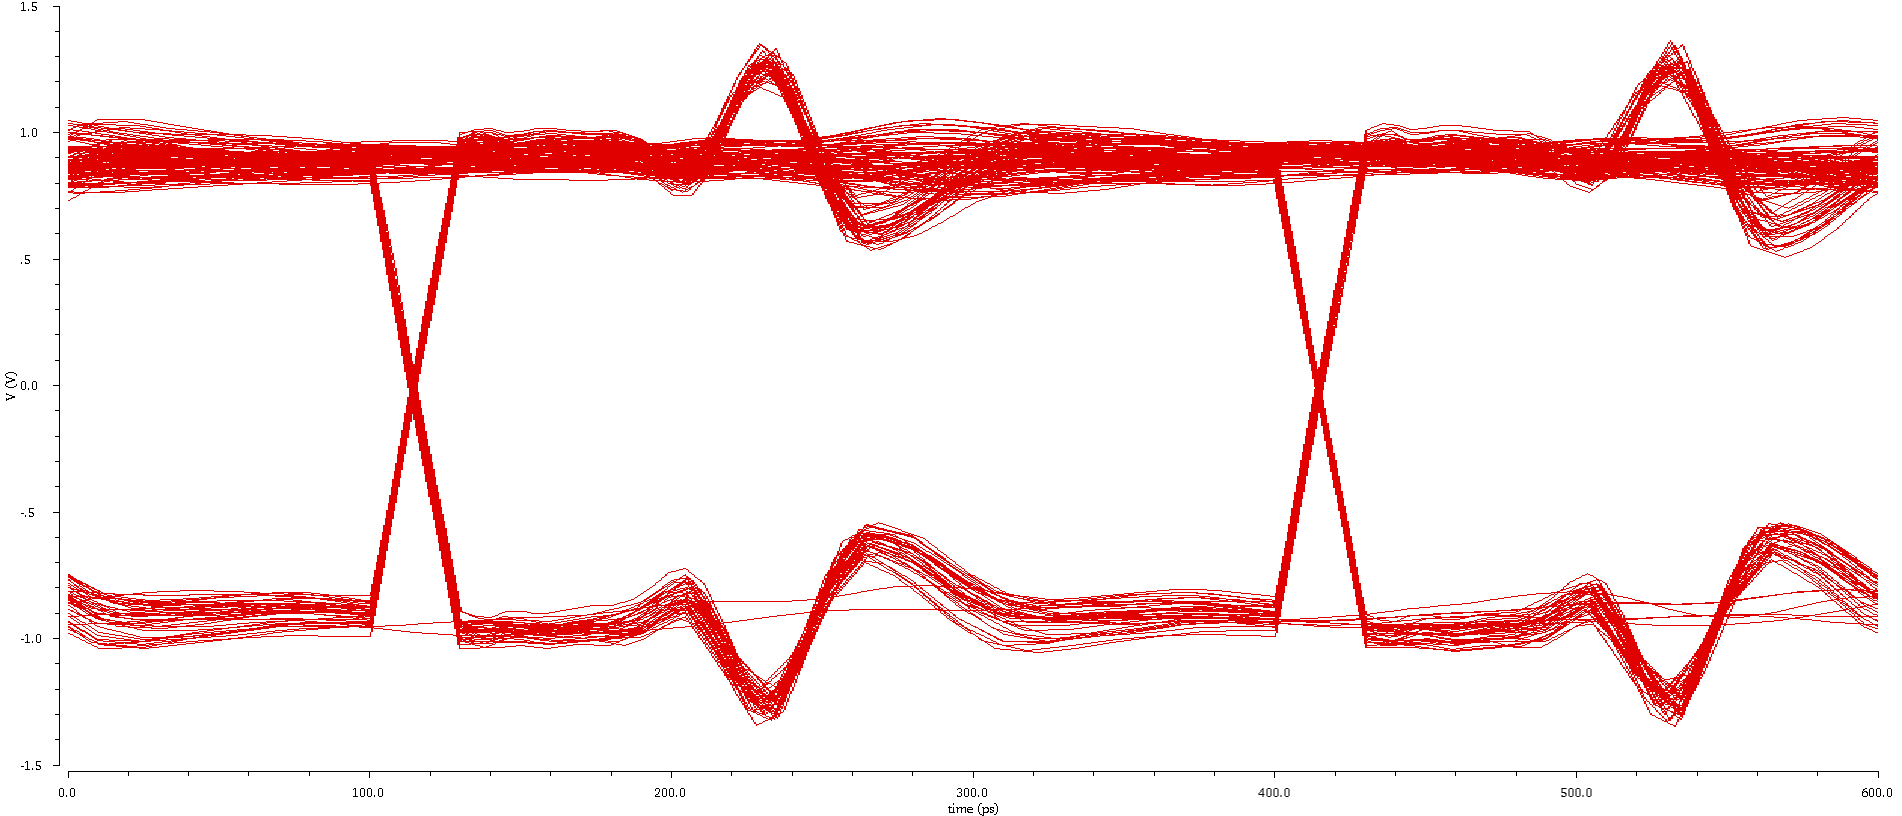
\includegraphics[width=\textwidth]{./img/channel_response_eye_diagram/3gbp_eye_total_before_channel.png}
		\subcaption{Simulated eye at 3Gbps at port A. \\ Eye width: 95\% eye height: 55\%.}
	\end{minipage}%	
	\begin{minipage}[tb]{0.5\textwidth}
		\centering	
		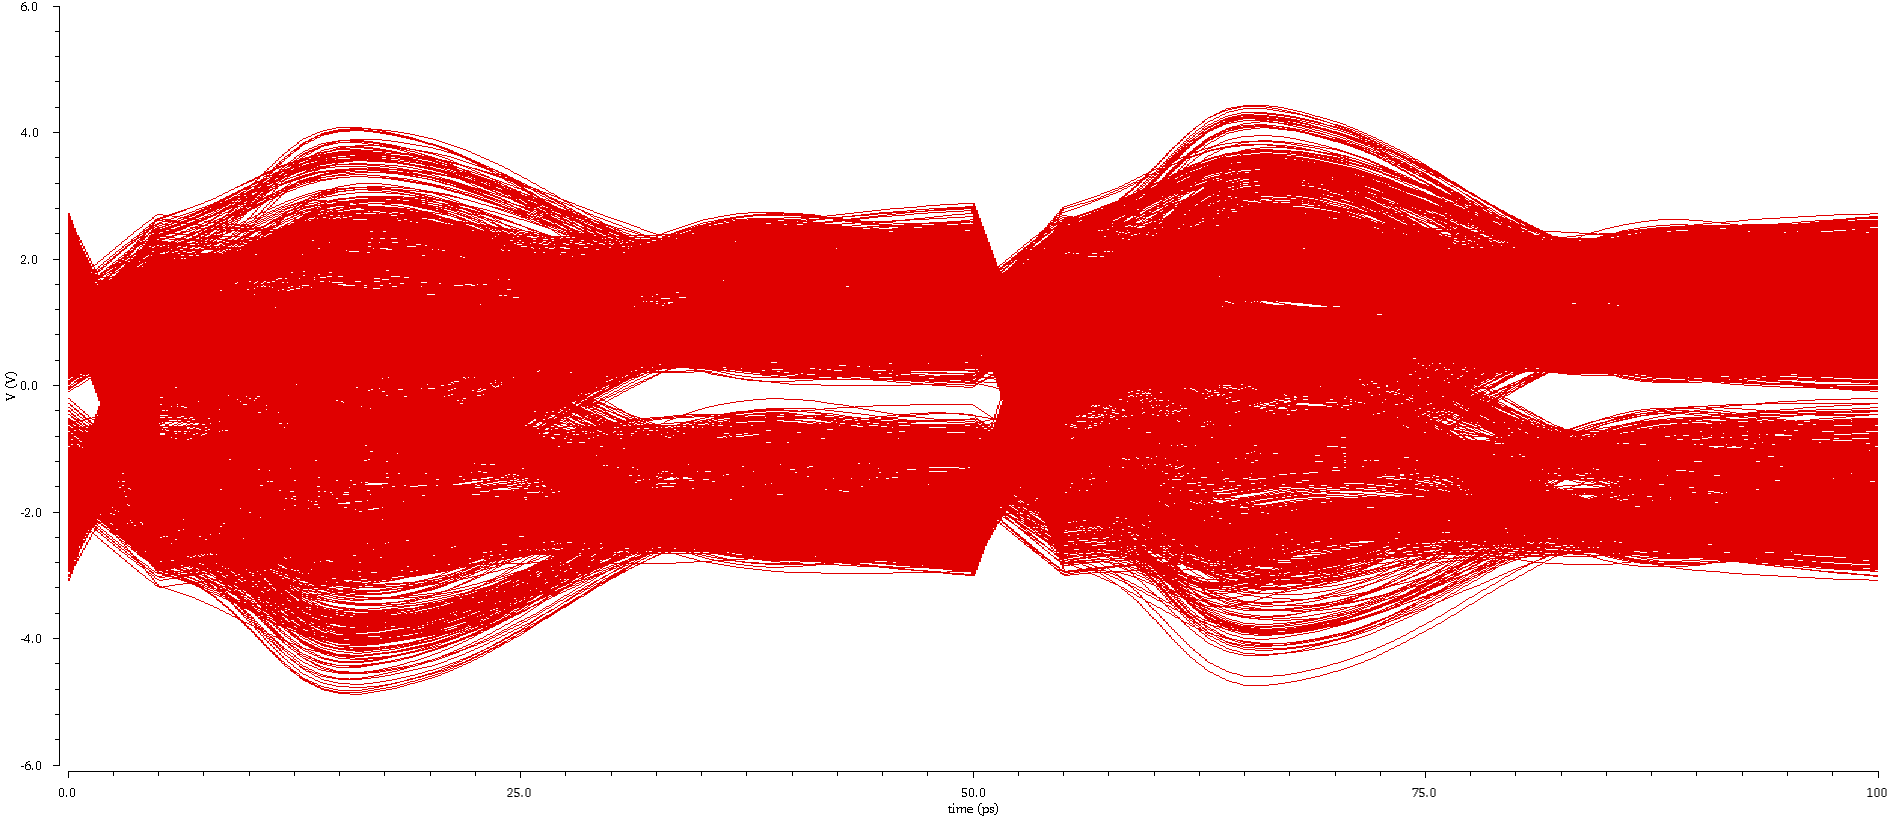
\includegraphics[width=\textwidth]{./img/channel_response_eye_diagram/20gbp_eye_total_before_channel.png}
		\subcaption{Simulated eye at 20Gbps at port A. \\ Eye closed.}
	\end{minipage}%
	\label{fig:eye_total_port_A}
	\caption{Simulated eye at port A.}
\end{figure*}

\begin{figure*}[htbp!]
	\captionsetup[subfigure]{justification=centering}
	\begin{minipage}[tb]{0.5\textwidth}
		\centering	
		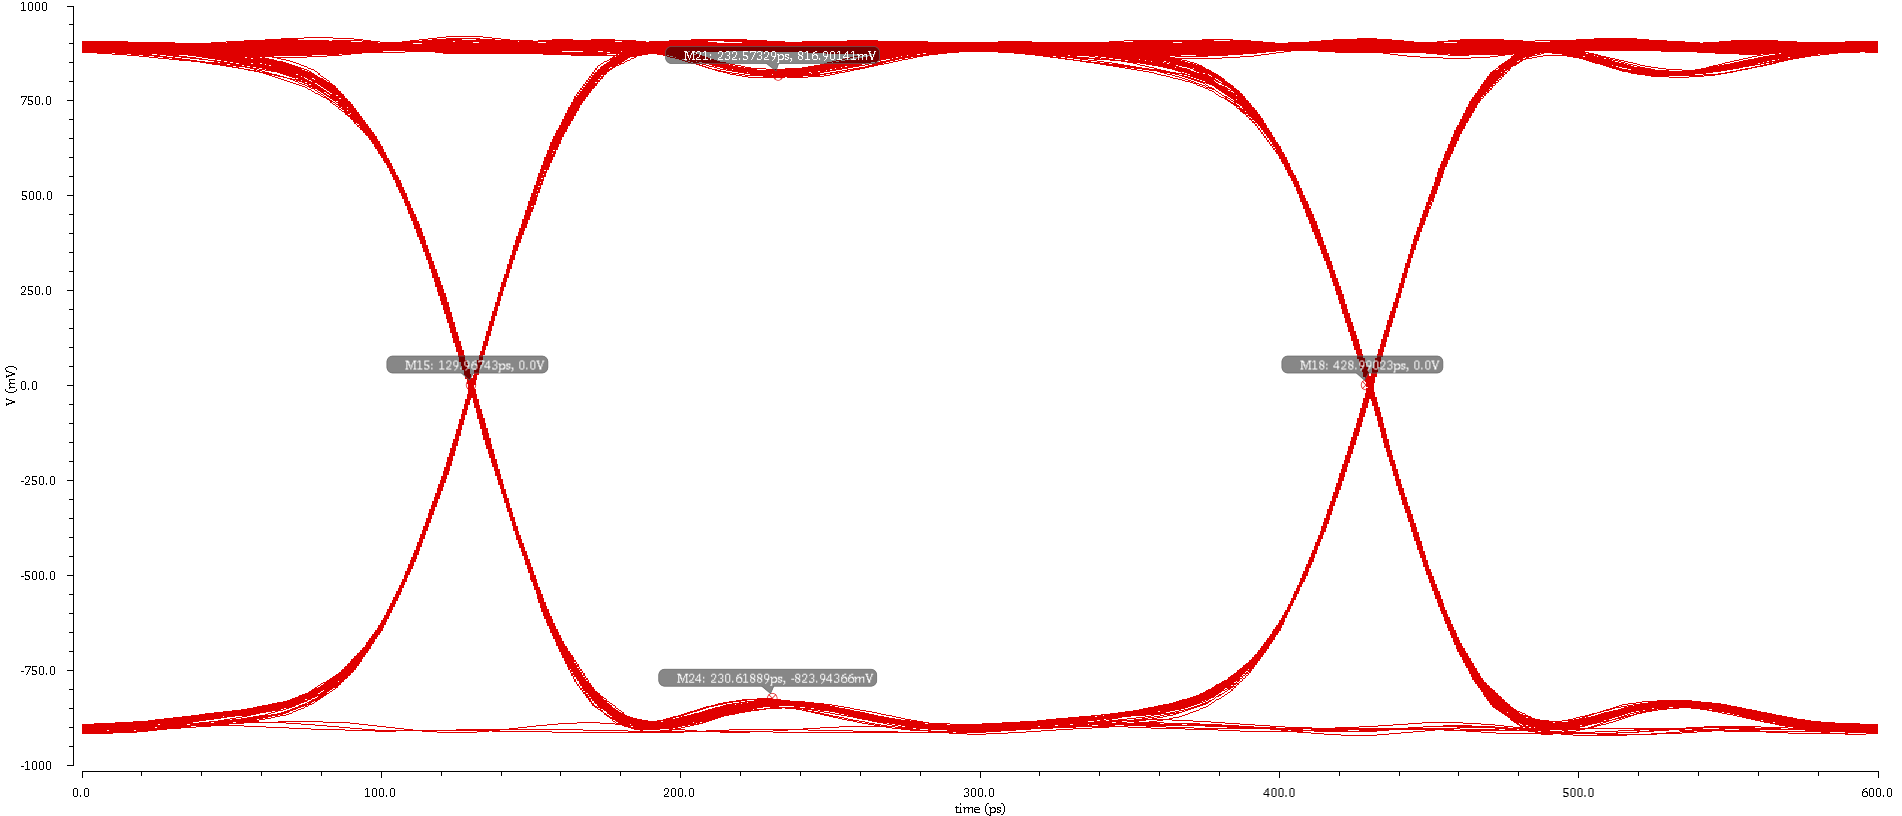
\includegraphics[width=\textwidth]{./img/channel_response_eye_diagram/3gbp_eye_total_before_dfe.png}
		\subcaption{Simulated eye at 3Gbps received at port B. \\ Eye width: 99\% eye height: 91\%.}
	\end{minipage}%	
	\begin{minipage}[tb]{0.5\textwidth}
		\centering	
		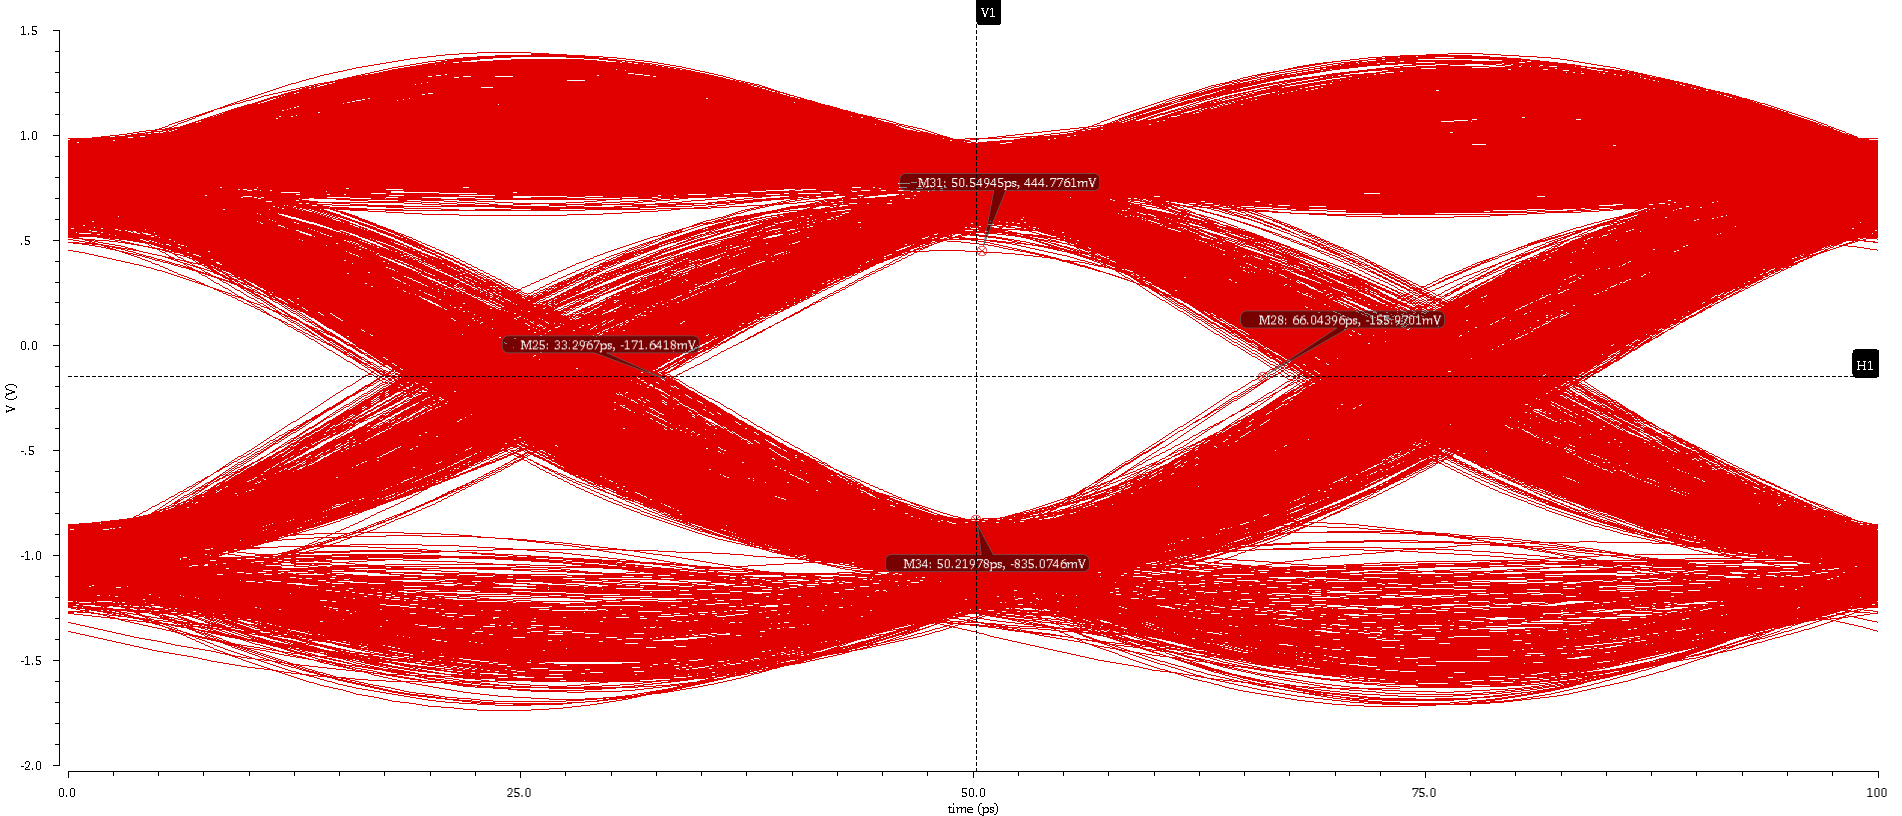
\includegraphics[width=\textwidth]{./img/channel_response_eye_diagram/20gbp_eye_total_before_dfe.png}
		\subcaption{Simulated eye at 20Gbps received at port B. \\ Eye width: 66\% eye height: 71\%.}
	\end{minipage}%
	\label{fig:eye_total_port_B}
	\caption{Simulated eye at port B.}
\end{figure*}

\begin{figure*}[htbp!]
	\captionsetup[subfigure]{justification=centering}
	\begin{minipage}[tb]{0.5\textwidth}
		\centering	
		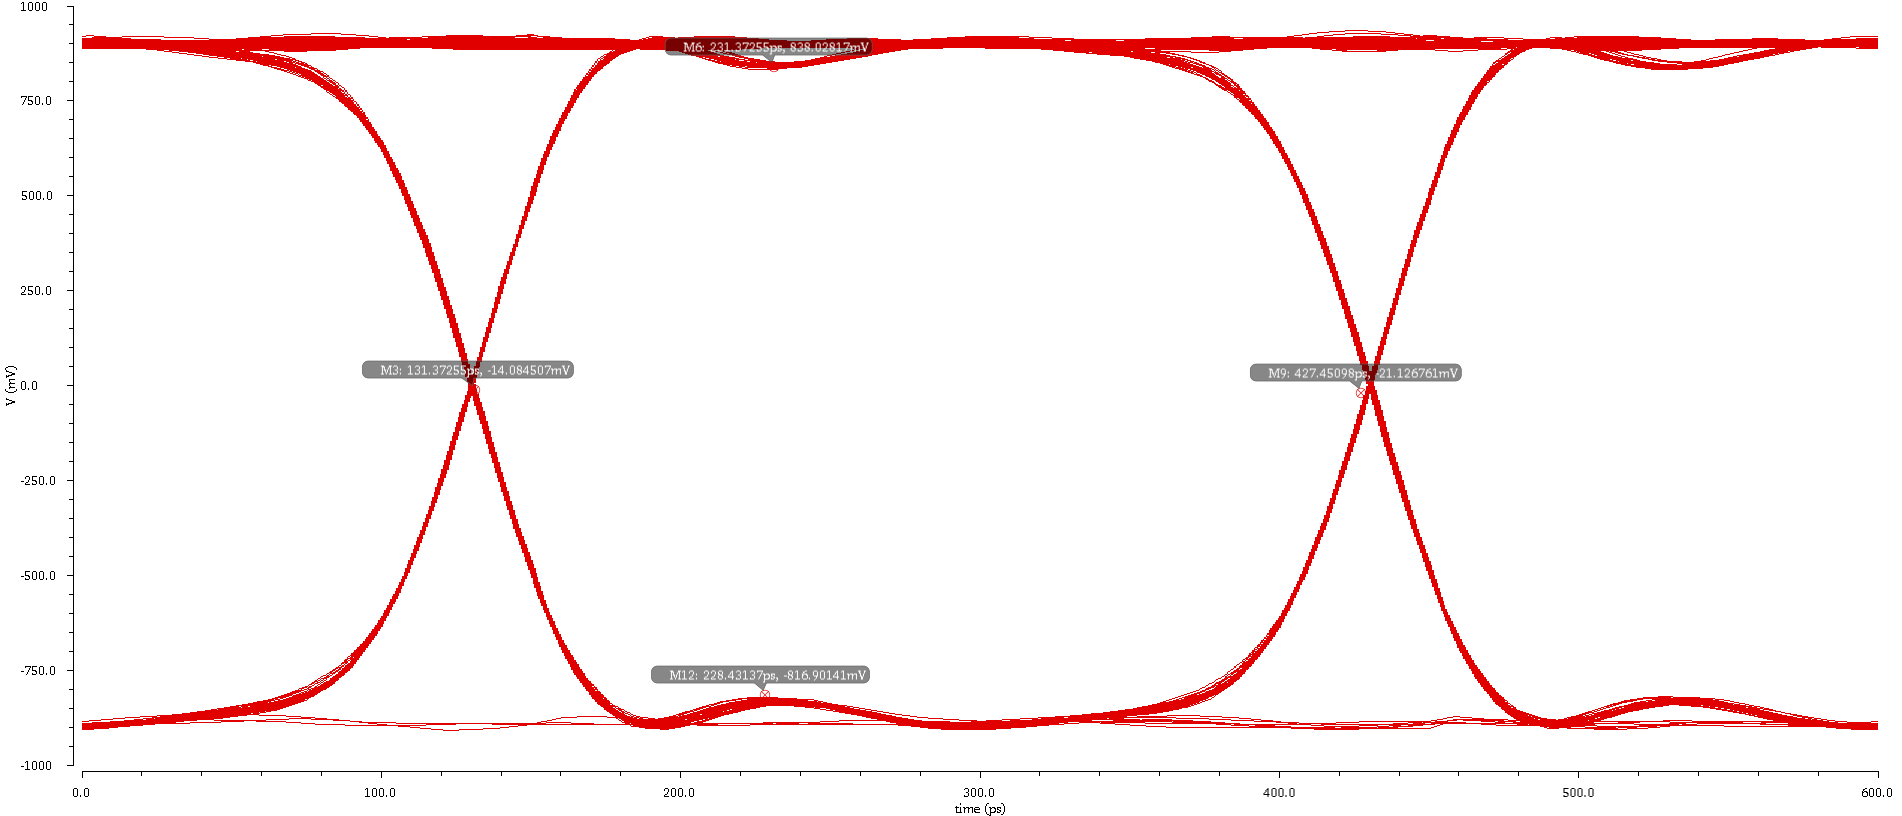
\includegraphics[width=\textwidth]{./img/channel_response_eye_diagram/3gbp_eye_total.png}
		\subcaption{Simulated eye at 3Gbps received at port C.\\ Eye width: 98\% eye height: 92\%.}
	\end{minipage}%	
	\begin{minipage}[tb]{0.5\textwidth}
		\centering	
		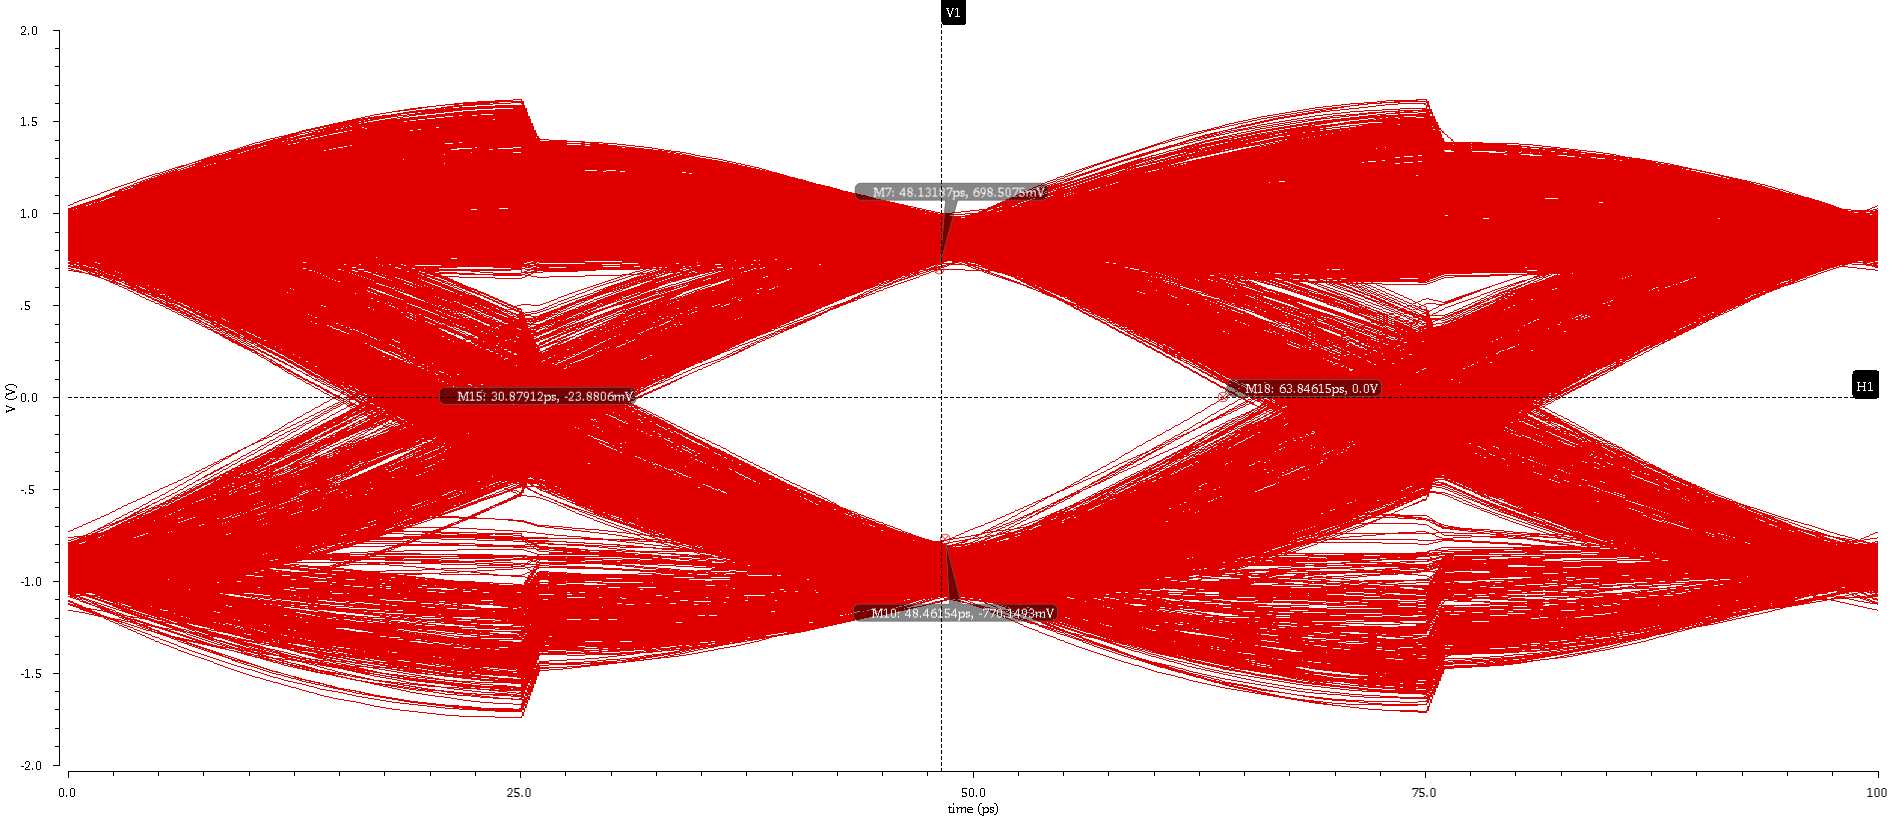
\includegraphics[width=\textwidth]{./img/channel_response_eye_diagram/20gbp_eye_total.png}
		\subcaption{Simulated eye at 20Gbps received at port C. \\ Eye width: 66\% eye height: 81\%.}
	\end{minipage}%
	\label{fig:eye_total_port_C}
	\caption{Simulated eye at port C. }
\end{figure*}

\section{Conclusion}
In this paper, we designed a passive channel with total length over 12 inches. The channel consists of package-to-PCB transition using bonding wire, and top-to-bottom via transition of PCB. This channel can achieve good performance subject to 3Gbps clock rate. With carefully designed FFE and DFE, this channel can further extends to 20Gbps. 

% =============  Reference Section ==============

\bibliographystyle{IEEEtran}
\bibliography{IEEEabrv,F:/SoftwarePC/AutoupdateZoteroLibrary}

%\begin{thebibliography}{99}	
%
%\end{thebibliography}

\end{paper}
\end{document}

